%!TEX program = xelatex
\documentclass[12pt]{report}
\usepackage[fontsize=13pt]{scrextend}
\usepackage[a4paper,top=2cm,bottom=2cm,left=3cm,right=2cm]{geometry}
% \usepackage{svg}
\usepackage{tgtermes}
\usepackage{fontspec}
\usepackage{biblatex}
\addbibresource{sections/ref.bib}
% \usepackage{pgfsys}
% \usepackage{transparent}
\setmainfont{Times New Roman}
\usepackage{eso-pic}
\usepackage{tikz}
\usepackage{fancyhdr}
\usepackage{lastpage}
\usepackage{tabularx}
\usepackage{amsmath}
\usepackage{amssymb}
\usetikzlibrary{positioning}
\usepackage{anyfontsize}
\usepackage{float}
\usepackage{titlesec}
\usepackage{listings}
\usepackage{lscape}
\linespread{1.5}
\usepackage{hyperref}
\usepackage{longtable}
\usepackage{xcolor}
\hypersetup{
    colorlinks,
    citecolor=black,
    filecolor=black,
    linkcolor=black,
    urlcolor=black
}
\usepackage{subcaption}

% Show subsections in the table of contents (TOC is the primary entry point for markers).
\setcounter{tocdepth}{2}
\setcounter{secnumdepth}{3}

\lstset{
    basicstyle=\small\ttfamily,
    numbers=left,
    frame=single,
}
\usepackage{pgfplots}
\pgfplotsset{compat=1.17}

\newcommand{\Khang}[1]{\textcolor{red!70!pink}{\textbf{\textit{#1}}}}

% Image placeholder macro.
% Usage: \imageplaceholder{Type}{What the image is}{How the author will capture it}
% Every figure in this report uses this macro so the author can fill in real images
% later. The master inventory of placeholders lives in Appendix C.
\newcommand{\imageplaceholder}[3]{%
  \begin{center}
  \fbox{\begin{minipage}{0.86\linewidth}
    \vspace{0.6cm}
    \centering
    \textbf{[IMAGE PLACEHOLDER]}\\[6pt]
    \begin{minipage}{0.92\linewidth}
      \raggedright
      \textit{Type:} #1\\[3pt]
      \textit{What:} #2\\[3pt]
      \textit{How to capture:} #3
    \end{minipage}\\
    \vspace{0.6cm}
  \end{minipage}}
  \end{center}
}

% Chapter title formatting.
\titleformat{\chapter}[display]{\normalfont\huge\bfseries}{\chaptertitlename\ \thechapter}{20pt}{\Huge}

\begin{document}

% sections/cover-page.tex

\begin{titlepage}
\AddToShipoutPictureBG*{%
    \AtPageLowerLeft{%
        \begin{tikzpicture}[overlay]
            \draw[line width=3pt]
            (3cm, 2cm) rectangle (\paperwidth-2cm, \paperheight-2cm);
            \draw[line width=1pt]
            (3.1cm, 2.1cm) rectangle (\paperwidth-2.1cm, \paperheight-2.1cm);
        \end{tikzpicture}%
    }%
}
\begin{center}
    \vspace*{0cm}
    \fontsize{15pt}{18pt}\selectfont
    \textbf{VIETNAM NATIONAL UNIVERSITY HO CHI MINH CITY}

    \textbf{HO CHI MINH CITY UNIVERSITY OF TECHNOLOGY}

    \textbf{FACULTY OF COMPUTER SCIENCE AND ENGINEERING}

    \begin{figure}[!htbp]
        \centering
        
\includegraphics[scale=0.3]{images/Logo_BK.png}
    \end{figure}

    \textbf{REPORT}

    \textbf{CAPSTONE PROJECT}

    \textbf{SEMESTER 252; ACADEMIC YEAR 2025--2026}

    \rule{0.8\textwidth}{0.5pt}

    \vspace{0.2cm}
    \fontsize{18pt}{24pt}\selectfont
    \textcolor{blue}{\textbf{\MakeUppercase{Studying and Developing Tools\\
    to Analyze and Visualize Bus Data}}}
    \vspace{0.2cm}

    \rule{0.8\textwidth}{0.5pt}
    \vspace{0.2cm}

    \fontsize{15pt}{18pt}\selectfont
    \textbf{MAJOR: COMPUTER SCIENCE}

    \vspace{0.4cm}

    \begin{tabular}{l l}
        \textbf{COUNCIL:}      & Assoc.\ Prof.\ Vo Thi Ngoc Chau \\
                               & M.Sc.\ Le Dinh Thuan \\
                               & Dr.\ Le Thanh Van \\
        \textbf{SUPERVISOR:}   & Assoc.\ Prof.\ Thoai Nam \\
    \end{tabular}

    \vspace{0.3cm}
    \textbf{------o0o------}
    \vspace{0.3cm}

    \begin{tabular}{l l}
        \textbf{STUDENT:} & Huynh Thanh Duy --- 2252114 \\
    \end{tabular}

    \vspace{0.2cm}
    \fontsize{14pt}{18pt}\selectfont
    HO CHI MINH CITY, June 2026
\end{center}
\end{titlepage}
\setmainfont{Times New Roman}

\clearpage
\pagenumbering{roman}
\chapter*{Instructor’s Signature}

\vspace{1cm}

\makebox[0.7\linewidth][l]{\hrulefill} Date: \makebox[0.2\linewidth][l]{\hrulefill}

    \begin{flushleft}
    Assoc.\ Prof.\ Thoai Nam (Instructor)\\
    Faculty of Computer Science and Engineering
    \end{flushleft}

\chapter*{Declaration of Authenticity}

I declare that I solely conducted this capstone project, under the supervision of Assoc.\ Prof.\ Thoai Nam at the Faculty of Computer Science and Engineering, Vietnam National University -- Ho Chi Minh City University of Technology.
 
\noindent I have taken care to properly acknowledge and document all external sources and references used in the project.

\noindent If there is any instance of plagiarism, I am ready to accept the consequences. Ho Chi Minh City University of Technology -- Vietnam National University HCMC will not be held responsible for any copyright violations that may have occurred during this research.

\vspace{2cm}

\begin{flushright}
\begin{tabular}{c}
    Ho Chi Minh City, June 2026 \\
    \textit{\textbf{Author,}} \\[0.3cm]
    Huynh Thanh Duy
\end{tabular}
\end{flushright}

\chapter*{Acknowledgement}

I would like to express my sincere gratitude to Assoc.\ Prof.\ Thoai Nam for his guidance throughout this project. His feedback on the system architecture, the analytical scope, and the structure of this report has been central to the work presented here.

\noindent I am grateful to the researchers who compiled and released the Ho Chi Minh City bus operational dataset used in this project, and to the open-source communities behind DuckDB, Polars, FastAPI, Plotly, and H3, whose tools underpin the implementation described in Chapter~\ref{chapter:implementation}.

\noindent I also thank the council members: Assoc.\ Prof.\ Vo Thi Ngoc Chau, M.Sc.\ Le Dinh Thuan, and Dr.\ Le Thanh Van for their time and evaluation.

\noindent Finally, I thank my family for their support and encouragement throughout this capstone project.


\chapter*{Abstract}
\addcontentsline{toc}{chapter}{Abstract}

Ho Chi Minh City operates a large public bus network whose Global Positioning System (GPS) telemetry and Automated Fare Collection (AFC) records produce a continuous stream of operational and demand data. The four existing public-facing tools available to residents (one route directory and three passenger routing applications) serve passenger navigation only; none of them provides analytical access to the network's performance, demand, or finance. The opening of the city's first metro line sharpens this gap by introducing an intermodal dependency between the bus network and the metro that the existing tools cannot monitor.

This report proposes an analytical and visualisation platform that integrates the two operational data streams behind a single queryable surface. The platform organises its analytical content into six themes (demand and crowding patterns, school-aware demand patterns, spatial and connectivity questions including bus-to-metro feeders, financial and operational efficiency, network-wide health and reliability, and per-route deep analysis). A four-layer warehouse stores raw views, conformed dimensions, fact views, and eight pre-computed aggregate tables, with the analytical surface reading exclusively from the aggregate layer to meet the interactive latency budget. The interaction model combines Multiple Coordinated Views (MCV) within each theme, an entity-detail interaction pattern on every clickable element, and the visual storytelling principles of Knaflic for chart presentation.

Phase One produces this report, four exploratory analysis notebooks (with field-level schema tables and five exploratory figures), a pixel-accurate user-interface mockup, and a partial implementation of the data-preprocessing pipeline at Layer 1 of the proposed architecture. The exploratory analysis finds that student fares account for approximately 34 percent of weekday-morning boardings, cash dominates payments at approximately 96 percent, route demand is heavy-tailed with the top 55 routes carrying 80 percent of total volume, and the Tết period produces a visible nine-day ridership trough.

The Phase Two implementation plan completes the warehouse and the analytical surface across nine sequential phases of approximately twenty-one working days, followed by a two-wave user evaluation across the four user roles. Three extensions are recorded as candidates for follow-on work: real-time arrival-time prediction, per-route anomaly detection, and bus telemetry as a city-wide traffic-sensing substrate.

\vspace{1em}
\noindent\textbf{Keywords:} public transit, bus operational analytics, visual analytics, multiple coordinated views, data warehouse.


\chapter*{Table of Glossary}
\addcontentsline{toc}{chapter}{Table of Glossary}

\begin{description}

\item[A1 (Linked brushing)] An invariant of the dashboard: within
a single card, selecting an entity in one chart highlights it in
every other chart of the same card. Implementation uses
Streamlit \texttt{session\_state} and \texttt{st.rerun()}.

\item[A2 (Story subtitle)] An invariant of the dashboard: every
chart carries a descriptive title \emph{and} a one-sentence story
subtitle that tells the viewer what to notice in the chart.

\item[A3 (Universal Entity Detail Panel)] An invariant of the
dashboard: every clickable entity (route, stop, school, company,
day, hour, hex cell, vehicle, driver) opens a side panel of
approximately forty percent of viewport with a multi-chart
mini-dashboard about that entity.

\item[AFC] Automated Fare Collection. The HCMC ticketing system
that logs each boarding event, the fare class, and the payment
channel. The local AFC dataset spans 1~January to 31~March~2026
with 17.8 million boarding records.

\item[Aggregate view] A pre-computed \texttt{CREATE OR REPLACE TABLE}
in DuckDB that serves one or more dashboard charts. The
warehouse defines eight aggregate views; every chart maps to
exactly one of them (the chart-to-aggregate data contract).

\item[BusLens] The product name of the visual analytics platform
delivered in this thesis.

\item[Card] One of the six themes in the dashboard hub
(School-Aware Demand, Demand \& Crowding, Spatial \& Connectivity,
Financial \& Operations, Network Health \& Performance, Routes).
Each card is anchored internally to one or two user roles but
presents the same chrome to every user.

\item[deck.gl HexagonLayer] A spatial-aggregation primitive that
bins boardings into hex cells of configurable radius
(200\,m / 500\,m / 1\,km) and colour-codes them by density.

\item[\texttt{dim\_route} canonical key] The AFC \texttt{route\_no}
field is the canonical \texttt{route\_id}; the GPS \texttt{route\_no}
is stored as a join field on \texttt{dim\_route}. Routes are
flagged as GPS-only or AFC-only where they appear in only one
source.

\item[Ghost run] A trip recorded in schedule data where GPS
positioning shows door openings on fewer than 20\% of scheduled
stops. Used as a proxy for operational waste in
Chart 4.1.

\item[Ghost stop] A stop that appears in the schedule but where
GPS logs show door openings on fewer than 20\% of scheduled
visits. Used in Chart 3.4.

\item[Gridify] A decoupling of data and visual grid abstractions
from Liu~(2022), used in the dashboard's hex-grid map layer.

\item[GroupSet / UpSet matrix] A set-intersection visualisation
from Liu~(2022) used in Chart~6.2 to show routes that belong to
multiple archetypes simultaneously (e.g., ``school AND
commuter'').

\item[HCMC Bus Analytics] The brand string shown in the dashboard
top bar.

\item[Hub $\rightarrow$ Card $\rightarrow$ Chart] The three-level
information-architecture hierarchy of the dashboard.

\item[Marey time--distance diagram] Chart 6.5; each trip on a
single route plotted as a diagonal line on a time-by-stop-distance
grid. Source: Lin~\&~Zeng (\cite{linzeng2014}).

\item[MCV (Multiple Coordinated Views)] An interaction model from
Liu~(2022) that the A1 linked-brushing invariant implements.

\item[QoS-1 / QoS-2 / QoS-3] Three Quality-of-Service tiers from
Srisakaokul~\textit{et~al.}~(\cite{srisakaokul2023}): QoS-1 = trip
completion, QoS-2 = on-path driving (50\,m route buffer), QoS-3
= on-schedule within tolerance~$T$.

\item[SDVF tiers] Solution-Decision-Value-Framework prioritisation
applied across the design space: FLAGSHIP (the differentiator) /
MUST (table-stakes) / SHOULD (depth) / COULD (secondary) / WON'T
(yet, scoped out for Phase~1).

\item[Stories layer] A scrollytelling section of the hub
presenting four curated narratives (The School Story, The
T\d ết~Story, The Money Story, The Network Map) on the same chart
canvases the cards expose.

\item[Threshold $T$] A tunable minutes-of-delay parameter for
anomaly detection in Chart 5.5. Pre-computed at $T \in
\{1, 2, 5, 10, 15\}$ minutes so the slider snaps between levels.

\end{description}


% \input{sections/list-of-abbreviations}

\tableofcontents

\listoftables
\newpage

\listoffigures
\newpage

\pagenumbering{arabic}

% ============================================================
% Chapter 1 — Introduction
% ============================================================
\chapter{Introduction}
\label{chapter:intro}

\textit{This chapter presents the motivation, scope, and outline
of the project. Contributions are summarised at the end of the
report in Chapter~\ref{chapter:conclusion} once the rest of the
report has established the context.}

\section{Motivation}
\label{sec:intro:motivation}
% sections/1.Introduction/1.1.Motivation.tex

\begin{figure}[H]
\centering
\imageplaceholder{Photograph}{A wide shot of an HCMC public bus on a busy
street, capturing the network in context (passengers boarding, route
signage visible)}{Photograph an HCMC bus during peak hours (e.g.,
District~1, B\'{e}n Th\`{a}nh area). Save as
\texttt{images/screenshots/hcmc\_bus\_photo.jpg}.}
\caption{The HCMC public bus network --- subject of this work.}
\label{fig:intro:bus}
\end{figure}

Ho Chi Minh City (HCMC) operates a bus network of approximately 152 urban
routes, 90 of which are subsidized, served by a fleet of over 2,000 vehicles
managed by the Centre for Public Transport Management~\cite{ttgtcc2024}.
Each day, the network's electronic ticketing system records every boarding
event, capturing when and where passengers tap in, what fare class they
pay, and which trip and vehicle they board. Combined with GPS positioning
and GTFS schedule data, this creates a detailed operational record of the
entire network's activity.
 
Despite this data richness, operational decisions are still largely driven by
manual inspection of spreadsheet exports and static reports. Anomalies that
are clearly visible in the data: a stop that is chronically delayed in the
evening peak, a route with an excessive proportion of near-empty trips, or a
bus that consistently misses the connection window at a metro interchange, go
undetected until they escalate into service failures. There is no unified,
interactive tool that allows a route administrator, a company executive, or a
city planner to explore the network's spatial and temporal dimensions without
data science expertise.

\begin{figure}[H]
\centering
\imageplaceholder{Screenshot}{The MCPT public route directory web page at
\url{buyttgtcc.com.vn} (or the official MCPT route lookup), showing a
list/table of routes with no analytical or aggregation
capability}{Open the MCPT public route directory in a browser, navigate
to the main route-list view, capture a full-page screenshot at a
typical viewport (e.g., 1440~px wide). Save as
\texttt{images/screenshots/mcpt\_directory.png}.}
\caption{The MCPT public route directory~\cite{ttgtcc2024} ---
the only operational artefact for the network publicly accessible
at the time of writing. The directory is a navigational tool,
not an analytical one: routes can be looked up but no aggregation,
visualisation, or temporal analysis is offered.}
\label{fig:intro:mcpt}
\end{figure}
 
This gap is further sharpened by the opening of Metro Line~1 on 22 December 2024~\cite{metro_wiki}, which
introduced an intermodal dependency into the network for the first time.
The effectiveness of metro-based urban mobility now depends directly on the
punctuality of bus feeder services: a bus arriving five minutes late at an
interchange station translates directly into a missed metro departure for its
passengers. Monitoring this intermodal relationship at scale requires
integrating bus operational data with the metro timetable, a capability absent
from existing management tools.

From an operational standpoint, transport companies and city administrators
face concrete daily questions that this data could answer but currently does
not: Which routes are running near-empty trips that waste fuel and driver
hours? Are scheduled trips actually departing on time, and if not, at which
stops does delay accumulate? Which routes carry disproportionate numbers of
subsidized passengers, including students and elderly riders, and are fare subsidies
reaching those groups efficiently? How does ridership shift between peak and
off-peak hours, and is the current trip frequency matched to actual demand?
Without interactive visualization tools, answering any of these questions
requires manual extraction and cross-referencing of multiple raw tables,
a process that is slow, error-prone, and inaccessible to non-technical staff.

This thesis develops \textbf{BusLens}, an analytics and visualisation
platform that reconciles the three data streams behind a single
queryable surface and exposes the network's spatial, temporal, and
financial dimensions through six themed lenses ---
\emph{Demand \& Crowding}, \emph{School-Aware Demand},
\emph{Spatial \& Connectivity}, \emph{Financial \& Operations},
\emph{Network Health \& Performance}, and \emph{Routes}. Each lens
is one card in an interactive hub
(Chapter~\ref{chapter:prototype}); each card is built on the same
data pipeline (Chapter~\ref{chapter:proposed}) and obeys three
invariants that anchor the user experience: linked brushing,
story-subtitled charts, and a universal entity detail panel that
opens on every entity click.

Looking ahead, the 2025--2030 bus network restructuring plan targets a
complete reorganisation of the current routes into a tiered hierarchy of
179 routes (18 trunk, 73 branch, 88 feeder)~\cite{vnexpress2023}, alongside
a full transition to electronic ticketing by 2025 and a 20--25\% electric
fleet by 2030~\cite{vnexpress2023}. These reforms will substantially increase
the volume and complexity of operational data-making the absence of visual
analytics tools an increasingly critical problem.



\section{Scope}
\label{sec:intro:scope}

The scope of this thesis is bounded along four axes: the data
sources analysed, the analytical questions addressed, the
stakeholders supported, and the deliverables produced.

\paragraph{Data scope.}
The analysis covers two complementary HCMC bus-network data streams:
GPS positioning data (a single-day local sample of 720{,}088 raw
pings from 2025-03-18 covering 9 routes; the full 50-day dataset of
$\sim$34\,GB referenced in the dataset specification~\cite{hcmcgps2025}
is reachable but not loaded locally), and AFC ticketing data
(17.9~million boarding events with paired payments over the 90-day
window 2026-01-01 to 2026-03-31). Static reference data --- stops,
routes, vehicles, companies --- is included as dimension tables.
The two streams are not joined by timestamp: their calendar windows
do not overlap. They are therefore treated as complementary sources
and combined narratively in the dashboard rather than fused at the
row level.

\paragraph{Analytical scope.}
Six classes of analytical question are in scope and one class is
explicitly out of scope. In scope:
(i)~system-wide demand and reliability (\emph{Network Health \&
Performance});
(ii)~when and where people ride (\emph{Demand \& Crowding});
(iii)~the network as a city map, including the bus--metro feeder
matrix (\emph{Spatial \& Connectivity});
(iv)~route profit-and-loss, payment-channel adoption, and
promotion impact (\emph{Financial \& Operations});
(v)~per-route deep-dive and cross-route clustering
(\emph{Routes}); and (vi)~the flagship lens on how universities
and schools shape demand (\emph{School-Aware Demand}). Out of
scope: real-time monitoring (the dashboard is historical-only),
individual passenger tracking (data killed it: 0.1\% of tickets
populate \texttt{user\_id}), passenger satisfaction (no survey
data exist), and natural-language SQL (delivered by an external
team).

\paragraph{Stakeholder scope.}
The dashboard is designed for four user roles, used internally as
a feature-prioritisation tool but not exposed in the UI:
\emph{passenger} (crowding, reliability, beginner-friendliness),
\emph{driver} (own shift, route detail),
\emph{company} (fleet performance, revenue, scorecard versus
network), and \emph{admin / MCPT} (network performance,
anomalies, equity, capacity). Each card is anchored internally to
one or two roles but exposes the same chrome to every user; no
role switcher, no role badges. The role-aware design is
implemented as feature prioritisation rather than separate views
so a stakeholder who needs cross-card context never has to leave
the tool.

\paragraph{Deliverables.}
Phase~1 produces four artefacts: (i)~this written report;
(ii)~four executed exploratory analysis notebooks
(\texttt{notebooks/01--04}) that ground every design decision in
the report; (iii)~the high-fidelity UI mockup at
\texttt{docs/design/app-layouts.html} that locks the dashboard's
visual language; and (iv)~the data-pipeline skeleton at
\texttt{src/duckdb\_loader.py} that already produces the
twenty-four raw views the warehouse design extends. The full
Streamlit application and the eight pre-computed aggregate views
are Phase~2 deliverables, scheduled per the implementation
roadmap in Chapter~\ref{chapter:future}.

\section{Thesis structure}
\label{sec:intro:structure}

The remainder of this thesis is organised into five further
chapters and three appendixes.

\paragraph{Chapter~\ref{chapter:background} --- Background and
Related Work.} Opens with a Related Work survey of the three
bodies of prior research the proposed solution builds upon ---
bus operational analytics, visualisation of spatial-temporal
traffic data, and existing HCMC analytical tools --- and then
develops the theoretical foundations the solution rests on: the
four-layer analytical warehouse, the DuckDB + Streamlit + Plotly
+ pydeck stack, the QoS scoring framework of
Srisakaokul~\textit{et al.}~\cite{srisakaokul2023}, the
visualisation primitives of Liu~\cite{liu2022}
(\emph{Gridify}, \emph{GroupSet}, \emph{FuzzyCut}) and the Marey
time--distance diagram of Lin~\&~Zeng~\cite{linzeng2014}, the
visual-storytelling principles of Knaflic~\cite{knaflic2015}, and
the Multiple Coordinated Views interaction model that the
dashboard's linked-brushing invariant implements.

\paragraph{Chapter~\ref{chapter:proposed} --- Proposed Solution.}
Opens with the problem statement, then develops the proposed
solution along five axes: an overview of the platform and its
solution-decision-value-framework prioritisation; the data
architecture (warehouse schema, conformed dimensions, fact and
aggregate views); the exploratory data analysis that scopes every
downstream design decision; the screening of analytical modules
against schema and EDA; and the dashboard specification (Hub
$\rightarrow$ Card $\rightarrow$ Chart hierarchy, six cards,
thirty-one canonical charts, three behavioural invariants, and
the scrollytelling Stories layer). This is the
highest-weighted chapter of the report (Câu~4 of the grading
rubric~\cite{rubric}, thirty points).

\paragraph{Chapter~\ref{chapter:prototype} --- Current Prototype.}
Presents the artefacts produced during Phase~1: the four
exploratory notebooks, the published high-fidelity UI mockup,
the data-pipeline skeleton, and the supporting design artefacts
that the Phase~2 implementation depends on.

\paragraph{Chapter~\ref{chapter:future} --- Future Work.}
Sketches the Phase~2 implementation roadmap (nine phases,
P1--P9, approximately twenty-one working days), the data
activations required to unlock currently-deferred features (full
50-day GPS, school geocoding), the predictive extensions that
follow naturally from the historical foundation
(arrival-time prediction, anomaly detection), and the planned
external integrations and user study. Together with
Appendix~B, this chapter addresses Câu~5 of the grading
rubric~\cite{rubric}.

\paragraph{Chapter~\ref{chapter:conclusion} --- Conclusion.}
Summarises the work, documents the four limitations that frame
its scope, enumerates the contributions of Phase~1, and closes
the report.

\paragraph{Appendixes.} Appendix~A documents the warehouse DDL
(table definitions for \texttt{dim\_route}, \texttt{dim\_date},
\texttt{fact\_boardings}, and \texttt{agg\_route\_hour}).
Appendix~B presents the Phase~2 plan as a phased schedule with
deliverables, dependencies, and expected outcomes per phase.
Appendix~C is the master inventory of every image and diagram
this report needs, with capture instructions for the author.


% ============================================================
% Chapter 2 — Background and Related Work
% (combines the old "Related Works" and "Theoretical Background" chapters;
% opens with a Related Work survey for Rubric Câu 3 coverage, then develops
% the theoretical foundations the proposed solution rests on.)
% ============================================================
\chapter{Background and Related Work}
\label{chapter:background}

\textit{This chapter surveys the prior research and the
theoretical foundations on which the proposed solution rests:
the bodies of related work that frame the problem (Câu~3 of the
grading rubric, see~\cite{rubric}), the four-layer warehouse
adaptation of the medallion data architecture, the analytical
stack that implements it, the QoS scoring framework, the
visualisation primitives borrowed from Liu and Lin~\&~Zeng, the
visual-storytelling principles of Knaflic, and the Multiple
Coordinated Views interaction model.}

\section{Related Work}
\label{sec:background:related}

\noindent\textit{This section surveys the prior research on
which the proposed solution rests. The grading rubric
(\cite{rubric}, Câu~3) requires at least three related problems
and at least three peer-reviewed studies; we identify four
distinct problem areas and seven supporting references, each of
which a later section of this chapter develops in technical
depth.}

\subsection{Bus operational analytics on GPS and AFC data}
\label{sec:background:related:ops}

The closest peer-reviewed work to the present thesis is
Srisakaokul~\textit{et~al.}'s study of public-city-bus service
quality in Bangkok~\cite{srisakaokul2023}, which derives three
quality-of-service tiers (QoS-1 trip completion, QoS-2 on-path
driving, QoS-3 on-schedule) from raw GPS pings and schedule
data. The framework transfers directly to the HCMC case and is
developed in Section~\ref{sec:theory:qos}.
A complementary line of research, exemplified by
Derevitskiy~\textit{et~al.}~\cite{derevitskiy2016}, treats the
bus fleet itself as a distributed traffic sensor: GPS pings are
aggregated into road-graph edge-speed estimates and propagated
to unsensed edges via macroscopic travel-time models. The
authors report a mean absolute percentage error around twenty
percent at distances under fifteen kilometres. The HCMC dataset's
fifty-day GPS window is in principle sufficient for the same
construction; the present thesis defers this extension to future
work (Section~\ref{sec:future:predictive}) in order to focus on
historical analytics in Phase~1.

A third line of work, Lin~\&~Zeng~\cite{linzeng2014}, builds a
real-time bus-arrival-time predictor on a link-node route
representation, with dwell at time-check stops as the dominant
predictor. The same time--distance trajectory construction
underlies the Marey diagram adopted in this thesis as the
Routes-card detail visualisation
(Section~\ref{sec:background:marey}).

\subsection{Visualisation of spatial--temporal traffic data}
\label{sec:background:related:viz}

The PhD work of Liu~\cite{liu2022} contributes three
visualisation primitives that the present thesis adopts
verbatim: \emph{Gridify} (a decoupling of data and visual grid
abstractions, used in the dashboard's hex-grid map),
\emph{GroupSet} (a set-intersection partitioning of routes by
archetype, used in the Routes card's UpSet matrix), and
\emph{FuzzyCut} (interactive categorisation). Liu also formalises
the Multiple Coordinated Views interaction model, which the
dashboard implements at full scope as the A1 linked-brushing
invariant of Chapter~\ref{chapter:proposed}.

A second body of work, the storytelling-with-data principles of
Knaflic~\cite{knaflic2015}, governs the chart-selection and
clutter-handling rules adopted in the dashboard. The A2 story
subtitle invariant of Chapter~\ref{chapter:proposed} is the
direct application of these principles as a design constraint
(no chart without a story subtitle; muted defaults; bright colour
reserved for the one element the story points at).

\subsection{Bus--metro intermodal connectivity and existing
HCMC tooling}
\label{sec:background:related:hcmc}

The advisor specification~\cite{thoai2025} names bus--metro
intermodal connectivity as a required feature of the dashboard
and supplies the table of nineteen bus routes that feed Metro
Line~1. The opening of Metro Line~1 on
22~December~2024~\cite{metro_wiki} sharpens the gap: the
effectiveness of urban metro mobility now depends on bus feeders
arriving on time at interchange stations, a connectivity
relationship the existing operational tools cannot monitor.

The principal existing HCMC analytical artefact is the MCPT
public route directory~\cite{ttgtcc2024}, which is a
navigational tool (routes can be looked up) but not an
analytical one (no aggregation, visualisation, or temporal
analysis). The HCMC dataset specification~\cite{hcmcgps2025}
documents the fifty-day GPS window of thirty-one routes and the
April~2025 parade week as a natural-experiment opportunity.
Together these references frame what the present thesis adds to
the local ecosystem: the first interactive analytical surface
over the network's GPS and AFC streams.

\section{Four-Layer Warehouse Adaptation}
\label{sec:background:warehouse}

The data architecture proposed in this thesis adopts the
\emph{medallion} pattern of Databricks~\cite{databricksMedallion}
as a conceptual template --- raw input, conformed intermediate
layers, and chart-ready output --- but specialises it to a
four-layer warehouse whose layer boundaries match the dashboard's
data needs.
\textbf{Layer~1} is the set of twenty-four raw views produced by
the upstream pipeline and registered by
\texttt{src/duckdb\_loader.py}.
\textbf{Layer~2} is a small star of ten conformed dimensions
(\texttt{dim\_date}, \texttt{dim\_route}, \texttt{dim\_stop},
\texttt{dim\_school}, \texttt{dim\_company},
\texttt{dim\_fare\_class}, \texttt{dim\_payment\_channel},
\texttt{dim\_vehicle}, \texttt{dim\_promotion},
\texttt{dim\_hour}) that reconciles the parallel GPS and AFC
identifier spaces and pre-tags the calendar with natural-experiment
windows (Tết, April-30 parade).
\textbf{Layer~3} is three fact views (\texttt{fact\_boardings},
\texttt{fact\_gps\_trips}, \texttt{fact\_stop\_visits}) that
re-shape the raw boarding and trip records through the conformed
dimensions.
\textbf{Layer~4} is the eight pre-computed aggregate tables that
feed the thirty-one dashboard charts: \texttt{agg\_route\_hour},
\texttt{agg\_route\_day}, \texttt{agg\_stop\_hour},
\texttt{agg\_school\_route}, \texttt{agg\_company\_route},
\texttt{agg\_payment\_day}, \texttt{agg\_network\_day}, and
\texttt{agg\_route\_profile}.

The specialisation collapses the classical Bronze-Silver-Gold
three-layer division into raw / dim / fact / agg because the
dashboard's chart catalogue defines a fixed, finite set of
aggregation grains. Pre-computing them once at warehouse-build
time replaces every other Gold-layer query the classical
pattern would otherwise need, and makes the chart-to-aggregate
mapping (Section~\ref{sec:proposed:modules}) a hard data contract
between the dashboard and the warehouse. The trade-off is that
adding a new chart at the last minute is no longer cheap; the
mitigation is the eight aggregate tables together absorb all but
one of the thirty-one charts in the catalogue (the only exception,
the Marey time--distance diagram of Chart~6.5, is built directly
on the fact layer because its grain is per-trip).

The whole warehouse fits in under one hundred megabytes of disk
and is held in DuckDB's columnar memory after first access, so
chart queries that read Layer~4 return in under twenty
milliseconds.

\section{Analytical Stack}
\label{sec:theory:stack}

A medallion pipeline can be implemented with many software
stacks, ranging from distributed Spark clusters to in-process
single-machine engines. This section introduces the four
classes of tool used in this work --- the analytical database,
the DataFrame runtime, the exploratory notebook environment,
and the visualisation libraries that drive a dashboard surface
--- with a brief description of each class and the specific
implementation chosen.

\subsection{DuckDB and Parquet}
\label{sec:theory:duckdb}

\imageplaceholder{Logo}{Logo of DuckDB}{Download the official logo of DuckDB from https://duckdb.org/; save as images/logos/duckdb.png}

\noindent
DuckDB~\cite{duckdb} is an in-process columnar SQL engine
purpose-built for analytical workloads on a single machine.
Three properties make it well-suited to a medallion
implementation. First, it reads Apache Parquet files
directly: a Parquet file on disk is queryable via
\texttt{read\_parquet('file.parquet')} without an explicit
\texttt{COPY} step. Second, it supports the SQL extensions an
analytical layer needs --- window functions,
\texttt{arg\_max()}, lateral joins, SQL macros for shared
expressions. Third, it has zero deployment overhead: no
separate server, no driver, no network round-trips, which
keeps any solution built on it reproducible from a single
\texttt{pip install}.

\medskip

Parquet is the on-disk format used at the Silver and Gold
layers. The format's columnar layout pairs naturally with the
projection-and-aggregation queries that analytical
applications issue, and ZSTD compression typically reduces raw
CSV by 5--10$\times$ on disk while preserving full query speed.

\subsection{Polars}
\label{sec:theory:polars}

\imageplaceholder{Logo}{Logo of Polars}{Download the official logo of Polars from https://pola.rs/; save as images/logos/polars.png}

\noindent
Polars~\cite{polars} is a high-performance DataFrame library
written in Rust with a Python API. It is the runtime used to
move data out of an analytical database and into application
code. The transfer happens over the Apache Arrow columnar
memory format, so a Polars DataFrame produced from a SQL query
shares memory with the underlying Arrow buffer and incurs no
copy. Polars also exposes a lazy expression API that pushes
filter and projection operations down into the underlying
engine, so the application only materialises the columns it
actually displays.

\subsection{Jupyter Notebook}
\label{sec:theory:jupyter}

\imageplaceholder{Logo}{Logo of Jupyter}{Download the official logo of Jupyter from https://jupyter.org/; save as images/logos/jupyter.png}

\noindent
Jupyter Notebook~\cite{jupyter} is a literate-computing
environment in which code, output, and prose live in the same
document. It is the canonical tool for exploratory data
analysis: the analyst writes a SQL or DataFrame expression,
runs it, inspects the result inline, and refines the next
query against what they just saw. Hypotheses verified
interactively in a notebook can later be promoted into a
materialised view in the Gold layer without rewriting the
underlying SQL. The notebook environment integrates natively
with both DuckDB and Polars.

\subsection{Streamlit}
\label{sec:theory:streamlit}

\imageplaceholder{Logo}{Logo of Streamlit}{Download the official logo of Streamlit from https://streamlit.io/; save as images/logos/streamlit.png}

\noindent
Streamlit~\cite{streamlit} is a Python framework for building
data applications with a reactive programming model. The
application is written as an ordinary Python script;
Streamlit re-executes the script on every user interaction and
renders the resulting widgets and figures to a browser. State
is held in a shared session-state object that survives across
re-executions. The reactive model is well-suited to MCV-style
dashboards (Section~\ref{sec:theory:mcv}) because filter
propagation reduces to writing a value to the session-state
object: every view that reads from that key re-renders
automatically.

\subsection{pydeck}
\label{sec:theory:pydeck}

\imageplaceholder{Logo}{Logo of pydeck}{Download the official logo of pydeck/deck.gl from https://deck.gl/; save as images/logos/pydeck.png}

\noindent
pydeck~\cite{pydeck} is the Python wrapper for deck.gl, a
WebGL-based geospatial visualisation library originally
released by Uber. It draws thousands of map features --- stop
dots, route polylines, catchment polygons --- at interactive
frame rates and exposes click events back to the host
application. The \texttt{ScatterplotLayer} used in this work
supports continuous colour gradients and per-point tooltips,
which are the two primitives a stop-density map requires.

\subsection{Plotly}
\label{sec:theory:plotly}

\imageplaceholder{Logo}{Logo of Plotly}{Download the official logo of Plotly from https://plotly.com/; save as images/logos/plotly.png}

\noindent
Plotly~\cite{plotly} is a charting library that provides the
canonical chart vocabulary --- line, area, bar, scatter,
treemap, histogram, box plot, heatmap --- used by analytical
dashboards. It supports server-side interactivity: click,
brush, and hover events are reported back to the host
application so that a chart click can trigger a state change
elsewhere. Plotly's chart catalogue covers every analytical
question identified in Chapter~\ref{chapter:proposed} without
extension.

\bigskip

The six tools above cover the entire analytical stack from raw
data to rendered dashboard. None is exotic; together they form
a small, maintainable surface area that can be deployed from a
single Python environment with no external services.

Of the thirty-one canonical charts specified in the dashboard
(Section~\ref{sec:proposed:dashboard}), twenty-two render
natively through \texttt{st.plotly\_chart}: heatmaps, ranked
bars, parallel coordinates, treemaps, scatter quadrants, stacked
areas, promotion-lift bars, and the demand-forecast multi-line
chart. Six charts use \texttt{st.pydeck\_chart} for deck.gl
integration: 3.1 network overview, 3.2 boarding density
HexagonLayer, 3.3 stop demand explorer, 3.4 ghost-stop map, 3.5
bus--metro feeder map, and 1.5 school proximity map. The
remaining three charts (6.1 the UMAP route constellation, 6.2
the GroupSet/UpSet archetype matrix, 6.5 the Marey
time--distance diagram), plus the hub landing page, the
scrollytelling Stories layer, and the universal entity-detail
panel (invariant~A3 of Section~\ref{sec:proposed:invariants}),
are injected via \texttt{st.components.v1.html} as self-contained
HTML components that own their own interactivity.

\input{sections/3.TheoreticalBackground/3.3.QoSScoring}
\section{Visualisation Primitives}
\label{sec:theory:primitives}

The thesis of Liu~\cite{liu2022} introduces three reusable
visualisation primitives for spatial-temporal data ---
\emph{FuzzyCut}, \emph{Gridify}, and \emph{GroupSet}. Each
primitive solves a recurring class of analytical problem and
each is generic enough to be applied to several different
underlying variables. This section presents each primitive in
its own terms.

\subsection{FuzzyCut}
\label{sec:theory:fuzzycut}

Many analytical questions ask the user to categorise a
continuous variable --- a speed, a fare, a duration --- into
qualitative bins such as \emph{Slow}, \emph{Normal} and
\emph{Fast}. The choice of cut-points is rarely obvious in
advance. Fixing the cut-points produces a brittle visualisation
that misclassifies values near the boundaries, and switching
the cut-points abruptly produces distracting visual jumps as
the analyst tunes the thresholds.

FuzzyCut addresses this with \emph{fuzzy} membership functions
over the variable's domain. Each value is assigned a partial
membership in each category according to a smooth membership
curve centred on the analyst's chosen cut-point; values exactly
at the cut-point belong half to one category and half to the
neighbouring category, and the membership transitions
continuously rather than abruptly. The analyst adjusts
cut-points by dragging interactive lines on a histogram of the
variable; downstream visualisations recolour in real time, with
smooth transitions in the boundary regions rather than discrete
jumps. Liu shows that fuzzy membership reduces the visual
instability of classical discrete bins and enables analysts to
discover stable threshold settings interactively.

The technique is application-agnostic. The same FuzzyCut
mechanism can categorise traffic speeds (\emph{Congested /
Slow / Normal / Fast}), revenue per trip (\emph{High / Medium
/ Low / Loss-making}), or any other continuous variable on
which a small number of qualitative bands are useful.

\subsection{Gridify}
\label{sec:theory:gridify}

Spatial accessibility analysis asks how easily a population
can reach a given resource. The canonical question is
\emph{how far is the average resident from the nearest active
resource?} A naive answer overlays resource dots on a base map,
but this conveys density rather than accessibility: the analyst
cannot tell which areas are underserved without computing
distances explicitly.

Gridify divides the geographic region of interest into a
regular grid of configurable cell size (typically tens to
hundreds of metres on a side). Each cell is coloured by an
aggregate over the points it contains --- in the accessibility
setting, the average distance from the cell centroid to the
nearest active resource. The grid abstraction transforms a
point-density question into a region-colouring question, which
is far easier to read at a glance. A time-of-day toggle
reveals how the colouring changes across the day, exposing
resources whose availability varies with the time at which the
question is asked.

Liu demonstrates Gridify on origin--destination flows in Lyon,
but the technique applies to any spatial accessibility question
in which the analyst needs to know not where the resources are
but where they are not.

\subsection{GroupSet}
\label{sec:theory:groupset}

A common analytical question across many domains is \emph{which
elements (routes, sensors, stops, stations) behave similarly
over time?} The analyst's instinct is often to cluster the
elements by their hourly or daily time-series, but classical
clustering algorithms require the analyst to specify the number
of clusters and to fix a distance metric in advance. The result
is a single static partition that is hard to adjust as the
analyst's understanding evolves.

GroupSet replaces the single static partition with an
interactive collection of editable sets. Each element is
assigned to an initial group based on its time-series shape;
the analyst can then merge groups by dragging them together,
split a group by selecting a subset of its members and
detaching them, or relabel a group with a domain term such as
\emph{AM Peak Only} or \emph{Chronically Empty}. The technique
preserves the analyst's qualitative judgements while still
benefitting from algorithmic suggestions about which elements
group naturally together. The result is a partition that the
analyst owns, in contrast to the partition that an opaque
clustering algorithm imposes.

\subsection{Marey time--distance diagram}
\label{sec:background:marey}

A fourth primitive used in this thesis is the Marey time--distance
diagram~\cite{linzeng2014}. The diagram plots, for each trip on a
single route, a polyline on a two-dimensional grid whose
horizontal axis is wall-clock time and whose vertical axis is the
ordinal position of each stop along the route. The slope of the
polyline at any point is the bus's local speed; a horizontal
segment indicates a dwell at a stop; the vertical gap between
two consecutive polylines is the headway between two buses at
the same point on the route. Bunching, the operational pathology
in which two scheduled buses converge in time, appears in the
diagram as two polylines that move from a separated state to a
converging state along the time axis. Schedule gaps appear as
wide horizontal voids in the diagram. The Routes card of this
thesis renders a Marey diagram as its principal Detail-mode chart
(Chart~6.5 of Section~\ref{sec:proposed:dashboard}).

\section{Visual Storytelling}
\label{sec:theory:storytelling}

The visualisation primitives of
Section~\ref{sec:theory:primitives} provide the technical
building blocks of a dashboard. Whether a chart built from
those blocks actually communicates with a stakeholder, however,
depends on a different body of practice --- visual
storytelling. Knaflic's \emph{Storytelling with
Data}~\cite{knaflic2015} is the foundational practitioner
reference; this section summarises the four principles from
that book that govern the visual design of analytical
dashboards.

\subsection{Choose the right chart for the question}

Knaflic argues that the analyst's first decision is the
\emph{type} of chart, and that the canonical chart type for
each analytical question is almost always the right choice.
Time series should be rendered as line or stacked-area charts,
distributions as histograms or box plots, two-variable
relationships as scatter plots, hierarchical part-of-whole as
treemaps, and categorical comparisons as horizontal bars. The
implication is that ornate alternatives --- 3D bars, gauges,
radial layouts --- whose decorative weight outpaces their
information content should be avoided. The analyst's attention
should be on the data and the analytical claim, not on the
novelty of the chart.

\subsection{Eliminate clutter}

Knaflic's second principle is that every visual element on a
chart competes for the analyst's attention; elements that do
not carry information should be removed. Concrete examples
include gridlines that double as axis tick-marks, axis labels
that duplicate what the chart title already says, legends
that duplicate already-visible labels, and decorative drop
shadows or gradients. The principle generalises to dashboard
chrome: filter widgets that show their default values, status
bars that are always green, and breadcrumb navigation that
never changes. Removing such elements is one of the cheapest
visual improvements a dashboard can make, because every
removal increases the relative weight of the remaining
elements.

\subsection{Direct attention}

Knaflic's third principle is that the analyst's eye should be
directed to the analytical claim of the chart, not to its
decorative chrome. Three techniques are most often used.
\emph{Pre-attentive attributes} --- colour, size, position ---
are reserved for the variables being foregrounded; everything
else uses neutral grey. A consistent \emph{colour role} is
maintained across charts: a single primary colour is reserved
for the variable being highlighted, and a diverging palette
(typically red--amber--green) is reserved for ``low / medium /
high'' scales. \emph{Annotation} draws the eye to specific
points: a single labelled callout on a long line chart is
worth more than a dense legend with the same information. The
common thread is that the analyst is told what to look at,
not asked to find it.

\subsection{Tell a story across the dashboard}

The fourth principle, and the one most specific to multi-view
dashboards, is that the analyst's progression from view to
view should follow a narrative. The interaction model
(Section~\ref{sec:theory:mcv}) is the mechanism, but the
narrative is a design choice. The canonical narrative is
\emph{aggregate $\rightarrow$ detail}: the analyst opens on a
high-level KPI, identifies an outlier, clicks to drill into
the outlying entity, inspects its components, and either
resolves the question or escalates back to the aggregate to
compare the entity against its peers. Knaflic frames this as
``drill-from-symptom-to-cause'' and argues that any dashboard
worth using must support it explicitly through one-click
navigation between views, not just through a side-by-side
layout that leaves the navigation up to the analyst.

The chart-design invariant of this thesis, denoted~A2 in
Section~\ref{sec:proposed:invariants}, applies these principles
verbatim: every chart in the dashboard carries a descriptive
title in neutral language and a one-sentence story subtitle in
emphasised type that tells the viewer what to notice in the
chart; default chart colours are kept muted, with saturated
colour reserved for the single element the story subtitle points
at; and chart annotations underline the same finding the subtitle
states.

\section{Multiple Coordinated Views}
\label{sec:theory:mcv}

The Multiple Coordinated Views (MCV) interaction
model~\cite{liu2022} is the principle that connects the
visualisation primitives of Section~\ref{sec:theory:primitives}
and the storytelling principles of
Section~\ref{sec:theory:storytelling} into a coherent
interactive dashboard.

An MCV system is a collection of views over a shared dataset,
with the property that any selection or filter applied in one
view propagates instantaneously to every other view. The
canonical implementation is \emph{brushing-and-linking}: a
brush stroke over one chart highlights the corresponding
regions in all other charts, and the highlight follows the
brush continuously as the analyst moves it. The model
formalises an intuition that has appeared in interactive
analytical systems for several decades; it provides the
vocabulary in which modern dashboard designs can be described
and compared.

\subsection{Implementation requirements}

An MCV system imposes three requirements on its implementation.
First, all views must share a single source of truth for filter
state, so that an update in one view is observable in all the
others without requiring view-to-view notification. Second,
the views must be independently rendered: if one view is
expensive to recompute it must not block the others. Third,
the navigation between views must be one-click rather than
menu-driven, so that analysts can shift their attention from
view to view at the speed of thought.

\subsection{The ControlCenter abstraction}

Liu introduces the \emph{ControlCenter} as the navigation
mechanism for MCV systems with many coordinated views. The
ControlCenter is a persistent UI element (typically an icon
strip or a docked panel) that allows the analyst to switch
between \emph{coordinated view sets} --- groups of views that
share analytical context --- while preserving the underlying
filter state. In Liu's traffic-control deployments the
ControlCenter appears at the left edge of the dashboard with
one icon per view set; clicking an icon swaps the visible
views without disturbing the filter context.

The ControlCenter resolves a long-standing tension in
multi-view dashboards: each analytical question wants its
own view set, but the analyst should not have to re-enter
filters every time they switch from one question to another.
The ControlCenter externalises the question selection from
the views themselves, so the dashboard can offer many
view sets without the cost of redundant filter chrome on each
one.

\subsection{Brushing-and-linking versus selection sharing}

Two flavours of MCV propagation appear in the literature.
\emph{Brushing-and-linking} highlights the same data points
across all views simultaneously: hovering a point on a scatter
plot illuminates the corresponding row in a table and the
corresponding region on a map. \emph{Selection sharing}
propagates a discrete selection event: clicking a tile in a
treemap commits a new value to the shared filter state, which
all views then re-render against. Brushing favours hover-driven
exploration; selection sharing favours click-driven drill-down.
A practical dashboard typically supports both, with brushing
on hover and selection sharing on click.

The dashboard implements MCV at full scope through what
Section~\ref{sec:proposed:invariants} denotes A1 linked brushing.
Within a single card, selecting an entity (a route row in a
heatmap, a bubble in a quadrant, a hex cell in a map) propagates
the selection to every other chart on the same card. The
implementation is server-side: a click writes to
\texttt{st.session\_state[\textquotesingle highlight\textquotesingle]},
\texttt{st.rerun()} triggers a re-render of all charts on the
page, and each chart reads the highlight on render. Cross-card
linking is reserved for explicit drill-down deep-links rather
than implicit propagation, to keep the per-card mental model
local.


% ============================================================
% Chapter 3 — Proposed Solution
% (THE highest-stakes chapter for marker review — 30 of 100 rubric points;
% opens with a Problem Statement section per advisor's instruction.)
% ============================================================
\chapter{Proposed Solution}
\label{chapter:proposed}

\textit{This chapter formalises the problem the project solves
and develops the proposed solution. It opens with a problem
statement, then presents the SDVF tier prioritisation, the
four-layer warehouse design, the empirical EDA findings that
ground every design decision, the module selection that screens
analytical modules against schema and data availability, and
the dashboard specification (Hub~$\rightarrow$~Card~$\rightarrow$~Chart
hierarchy, six cards, thirty-one canonical charts, three
behavioural invariants, and the scrollytelling Stories layer).}

\section{Problem Statement}
\label{sec:proposed:problem}

\noindent\textit{Stub --- this section formalises the
engineering problem the project solves, addressing
Câu~2 of the grading rubric (\cite{rubric}). Content
to be filled by subagent~E1.}

\section{Overview}
\label{sec:proposed:overview}

This chapter presents the proposed solution. It is developed in
four steps. Section~\ref{sec:proposed:dataarch} formalises the
data architecture --- both the schema across the GPS and AFC
source systems and the pipeline that produces the
pre-aggregated views the dashboard consumes.
Section~\ref{sec:proposed:eda} reports the exploratory data
analysis on the available HCMC sample, the findings of which
scope every downstream design decision.
Section~\ref{sec:proposed:modules} screens the analytics
modules drafted in the brainstorming phase against the schema
and the EDA findings, separating the modules that the local
data supports from those that require additional data
releases. Section~\ref{sec:proposed:dashboard} specifies the
dashboard: stakeholders and their analytical questions, filter
flexibility, the three-column layout, the canvas-swap
interaction, and the chart catalogue per analytical lens.

The solution rests on the theoretical foundations introduced
in Chapter~\ref{chapter:theory}: the medallion data
architecture, the analytical stack of DuckDB, Polars,
Streamlit, pydeck and Plotly, the three QoS indicators of
Srisakaokul~\textit{et al.}~\cite{srisakaokul2023}, the
FuzzyCut, GroupSet and Gridify visualisation primitives of
Liu~\cite{liu2022}, the visual storytelling principles of
Knaflic~\cite{knaflic2015}, and the Multiple Coordinated Views
interaction model. Where the local sample makes a literature
method only partially applicable (notably the GPS-side QoS
indicators which the local one-day sample limits), the
limitation is documented at the corresponding module rather
than silently bypassed.

\section{Data Architecture}
\label{sec:proposed:dataarch}

The data architecture has two complementary halves. The
\emph{schema} (Section~\ref{sec:proposed:schema}) describes what
tables exist and how they relate. The \emph{pipeline}
(Section~\ref{sec:proposed:pipeline}) describes how those tables
are produced from the raw exports and at what quality tier each
table sits. The two halves together replace four ad~hoc CSV
collections with a single queryable surface that the dashboard
draws from.

\subsection{Schema}
\label{sec:proposed:schema}

The HCMC dataset arrives as two parallel relational systems --- a
GPS-side schema produced by the vehicle telemetry system, and an
AFC-side schema produced by the fare-collection system --- plus a
small set of shared master tables. The relationships between the
two sides and the shared masters are shown in
Figure~\ref{fig:proposed:schema}.

\begin{figure}[H]
\centering
\begin{tikzpicture}[
    tbl/.style       ={rectangle, draw=#1, fill=#1!8,
                        rounded corners=2pt,
                        font=\scriptsize\sffamily,
                        align=left, inner sep=4pt,
                        text width=3.6cm},
    hdr/.style       ={rectangle, draw=#1, fill=#1!22,
                        rounded corners=2pt at top,
                        font=\scriptsize\sffamily\bfseries,
                        text width=3.6cm, align=center,
                        inner sep=2pt, minimum height=12pt},
    fk/.style        ={-stealth, blue!50!gray, dashed, thin},
    arrow/.style     ={-stealth, gray!60, thick},
    column/.style    ={font=\scriptsize\sffamily\bfseries\itshape,
                       color=gray!60!black},
    node distance=3pt and 6pt
]

\node[column] at (-5.0, 5.6) {GPS side};
\node[column] at ( 0.0, 5.6) {AFC side};
\node[column] at ( 5.0, 5.6) {Shared masters};

% --- GPS side ---
\node[hdr=orange!70!black]                       (h1) at (-5.0, 4.8) {gps\_trips};
\node[tbl=orange!70!black, below=0pt of h1]      (t1)
    {\textbf{PK} trip\_id\\\textbf{FK} route\_id, vehicle\_id\\start\_time, end\_time\\travel\_time, direction};

\node[hdr=orange!70!black, below=4pt of t1]      (h2) {gps\_stop\_times};
\node[tbl=orange!70!black, below=0pt of h2]      (t2)
    {\textbf{FK} trip\_id, station\_id\\arrival\_time, dwell\_time\\departure\_time, order};

\node[hdr=orange!70!black, below=4pt of t2]      (h3) {gps\_extracted};
\node[tbl=orange!70!black, below=0pt of h3]      (t3)
    {\textbf{FK} trip\_id\\ver\_lat, ver\_lng\\nearest\_stop\_id\\in\_buffer, hmm\_state};

\node[hdr=orange!70!black, below=4pt of t3]      (h4) {gps\_routes / schedules};
\node[tbl=orange!70!black, below=0pt of h4]      (t4)
    {route\_id, route\_no\\headway, distance\\departure / arrival times};

% --- AFC side ---
\node[hdr=blue!70!black]                         (a1) at (0.0, 4.8) {tickets};
\node[tbl=blue!70!black, below=0pt of a1]        (ta1)
    {\textbf{PK} ticket\_id\\\textbf{FK} trip\_id, station\_id\\ticket\_type\\time\_created\_ticket};

\node[hdr=blue!70!black, below=4pt of ta1]       (a2) {payments};
\node[tbl=blue!70!black, below=0pt of a2]        (ta2)
    {\textbf{PK} ticket\_id\\final\_price\\payment\_method};

\node[hdr=blue!70!black, below=4pt of ta2]       (a3) {ticket\_trips};
\node[tbl=blue!70!black, below=0pt of a3]        (ta3)
    {\textbf{PK} trip\_id\\\textbf{FK} route\_id, bus\_id\\direction};

\node[hdr=blue!70!black, below=4pt of ta3]       (a4) {ticket\_routes};
\node[tbl=blue!70!black, below=0pt of a4]        (ta4)
    {route\_id, route\_no\\\textbf{FK} company\_id};

% --- Shared ---
\node[hdr=green!50!black]                        (s1) at (5.0, 4.8) {stops\_master};
\node[tbl=green!50!black, below=0pt of s1]       (ts1)
    {stop\_id, stop\_name\\lat, lng, ward, zone\\type, routes\\(4\,710 HCMC stops)};

\node[hdr=green!50!black, below=4pt of ts1]      (s2) {ticket\_stations};
\node[tbl=green!50!black, below=0pt of s2]       (ts2)
    {station\_id\\station\_name\\lat, lng};

\node[hdr=green!50!black, below=4pt of ts2]      (s3) {gps\_stations};
\node[tbl=green!50!black, below=0pt of s3]       (ts3)
    {station\_id\\name, lat, lng\\type, zone};

% Within-side FK arrows
\draw[fk] (t1.south) -- (t2.north);
\draw[fk] (t1.east)  to[bend right=25] (t3.east);
\draw[fk] (t4.north) to[bend right=20] (t1.south);

\draw[fk] (ta1.south) -- (ta2.north);
\draw[fk] (ta1.east)  to[bend right=10] (ta3.east);
\draw[fk] (ta3.south) -- (ta4.north);

% Cross-side via shared masters (name-only match)
\draw[fk, dotted] (t2.east)  -- (ts3.west);
\draw[fk, dotted] (ta1.east) -- (ts2.west);
\draw[fk, dotted] (ts1.west) to[bend left=10]  (ts2.west);
\draw[fk, dotted] (ts1.west) to[bend right=10] (ts3.west);

\end{tikzpicture}
\caption{Data schema. GPS-side tables (left, orange) are keyed on
\texttt{trip\_id} and \texttt{vehicle\_id}; AFC-side tables
(centre, blue) are keyed on \texttt{ticket\_id} and a separate
\texttt{trip\_id}; the shared master tables (right, green)
connect the two sides only by stop-name lookup. Solid dashed
arrows are foreign-key relationships; dotted arrows are
name-only matches.}
\label{fig:proposed:schema}
\end{figure}

The GPS side captures every aspect of bus operation that can be
observed from vehicle telemetry. \texttt{gps\_raw} (not shown
above for compactness) holds the raw ping stream; the data
provider pre-aggregates the pings into \texttt{gps\_trips} (one
row per detected trip), \texttt{gps\_stop\_times} (one row per
stop visit within a trip), and \texttt{gps\_extracted} (the
HMM-filtered ping stream that QoS-2 consumes). The dimension
tables \texttt{gps\_routes}, \texttt{gps\_stations} and the
planned \texttt{gps\_schedules} carry the static reference data
that QoS-1 and QoS-3 require.

The AFC side records every boarding event. \texttt{tickets}
holds one row per scan, \texttt{payments} carries the financial
side keyed on \texttt{ticket\_id}, and \texttt{ticket\_trips}
provides per-trip metadata. The dimension tables
\texttt{ticket\_routes}, \texttt{ticket\_stations},
\texttt{ticket\_companies}, \texttt{ticket\_buses}, and the
route-stop sequence table \texttt{ticket\_route\_stops} complete
the side.

Two shared master tables sit alongside the side-specific
schemas. \texttt{stops\_master} is the HCMC-wide stop directory
(4{,}710 stops with names, latitude/longitude, ward, zone, and
the list of routes serving each stop). \texttt{vehicle\_route\_mapping}
provides an anonymised vehicle-hash to route-number lookup. The
two side-specific schemas cannot be joined by timestamp because
the GPS sample covers 2025-03-18 (single day) while the AFC
sample covers 2026-01-01 to 2026-03-31 (90 days, no overlap), and
a \texttt{vehicle\_id} bridge is unavailable: the GPS side uses
license-plate identifiers while the AFC side uses internal
\texttt{bus\_id} codes. The schema is therefore reconciled
narratively at the stop level via \texttt{stops\_master}
stop-name matching, rather than at the trip level.

\subsection{Pipeline}
\label{sec:proposed:pipeline}

The pipeline implements the medallion pattern of
Section~\ref{sec:theory:medallion} over the schema above. It
runs once at load time and produces the pre-aggregated
Gold-layer views the dashboard queries during interactive use.
Figure~\ref{fig:proposed:pipeline} shows the end-to-end flow.

\begin{figure}[H]
\centering
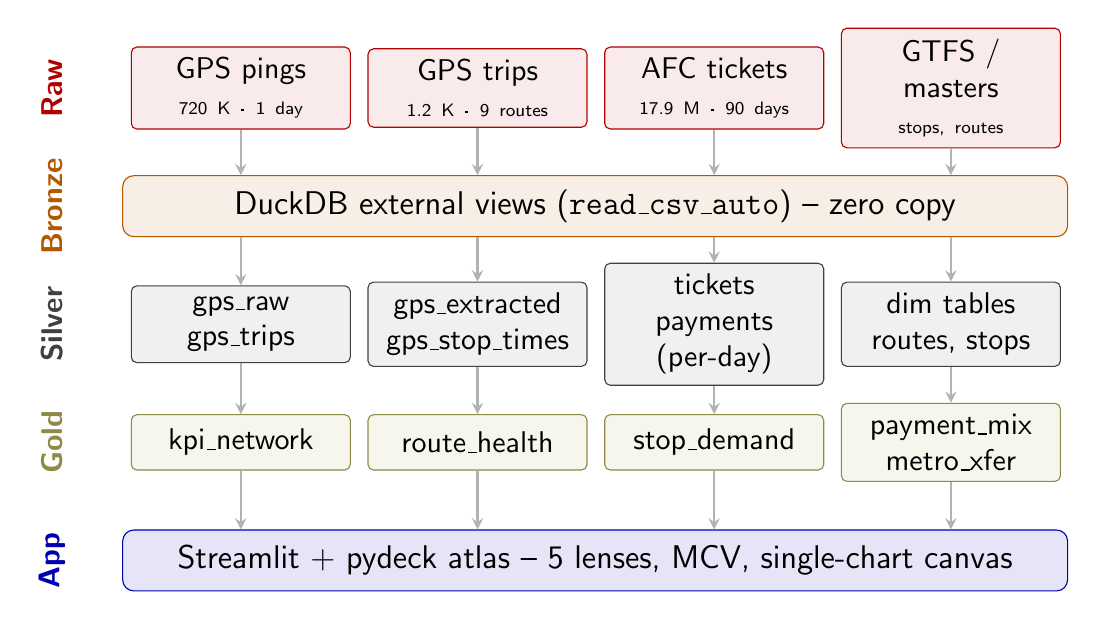
\begin{tikzpicture}[
    layer/.style    ={rectangle, rounded corners=4pt, draw=#1,
                       fill=#1!10, minimum height=22pt,
                       inner sep=4pt, font=\small\sffamily,
                       align=center},
    box/.style      ={rectangle, rounded corners=2pt, draw=#1,
                       fill=#1!8, minimum height=20pt,
                       inner xsep=4pt, font=\footnotesize\sffamily,
                       text width=2.5cm, align=center},
    label/.style    ={font=\footnotesize\sffamily\bfseries,
                       rotate=90, anchor=center},
    arrow/.style    ={-stealth, thick, draw=gray!60},
    node distance=3pt and 6pt
]

\node[label, color=red!70!black] at (-7.4, 4.6) {Raw};
\node[box=red!70!black] (r1) at (-5,4.6) {GPS pings\\\tiny 720 K · 1 day};
\node[box=red!70!black, right=of r1] (r2) {GPS trips\\\tiny 1.2 K · 9 routes};
\node[box=red!70!black, right=of r2] (r3) {AFC tickets\\\tiny 17.9 M · 90 days};
\node[box=red!70!black, right=of r3] (r4) {GTFS / masters\\\tiny stops, routes};

\node[label, color=orange!70!black] at (-7.4, 3.1) {Bronze};
\node[layer=orange!70!black, minimum width=12cm] (b) at (-0.5, 3.1)
    {DuckDB external views (\texttt{read\_csv\_auto}) -- zero copy};

\node[label, color=gray!50!black] at (-7.4, 1.6) {Silver};
\node[box=gray!50!black] (s1) at (-5,1.6) {gps\_raw\\gps\_trips};
\node[box=gray!50!black, right=of s1] (s2) {gps\_extracted\\gps\_stop\_times};
\node[box=gray!50!black, right=of s2] (s3) {tickets\\payments\\(per-day)};
\node[box=gray!50!black, right=of s3] (s4) {dim tables\\routes, stops};

\node[label, color=yellow!50!black] at (-7.4, 0.1) {Gold};
\node[box=yellow!50!black] (g1) at (-5,0.1) {kpi\_network};
\node[box=yellow!50!black, right=of g1] (g2) {route\_health};
\node[box=yellow!50!black, right=of g2] (g3) {stop\_demand};
\node[box=yellow!50!black, right=of g3] (g4) {payment\_mix\\metro\_xfer};

\node[label, color=blue!70!black] at (-7.4, -1.4) {App};
\node[layer=blue!70!black, minimum width=12cm] (app) at (-0.5, -1.4)
    {Streamlit + pydeck atlas -- 5 lenses, MCV, single-chart canvas};

\foreach \i in {r1,r2,r3,r4} \draw[arrow] (\i.south) -- (\i.south |- b.north);
\foreach \i in {s1,s2,s3,s4} \draw[arrow] (\i.north |- b.south) -- (\i.north);
\foreach \i/\j in {s1/g1, s2/g2, s3/g3, s4/g4} \draw[arrow] (\i.south) -- (\j.north);
\foreach \i in {g1,g2,g3,g4} \draw[arrow] (\i.south) -- (\i.south |- app.north);

\end{tikzpicture}
\caption{Five-layer pipeline. Bronze exposes raw files as
zero-copy DuckDB views; Silver materialises cleaned Parquet;
Gold pre-aggregates one table per analytical question; the app
layer consumes Gold for dashboard rendering.}
\label{fig:proposed:pipeline}
\end{figure}

\paragraph{Raw layer.}
The raw layer is the on-disk dataset as delivered. GPS data is
supplied as one CSV per day in \texttt{gps/raw\_gps/}; the local
sample is 720{,}088 rows for 2025-03-18. HMM-filtered per-trip
CSVs are provided under \texttt{extracted\_trips\_buffer\_50m/}
for the nine routes that GPS coverage extends to. AFC ticketing
data covers 90 days under \texttt{tickets/\{month\}/} and is
split into a tickets table (17.9~million rows) and a payments
table keyed on \texttt{ticket\_id}. Static reference data is
small and loaded as plain CSV. The raw files total approximately
3.3~GB on disk before compression.

\paragraph{Bronze layer.}
The Bronze layer registers DuckDB external views directly
against the raw files using \texttt{read\_csv\_auto} with
\texttt{ignore\_errors=true} and \texttt{union\_by\_name=true}.
No transformation occurs at this layer. Its purpose is to enable
schema inspection, ad~hoc SQL exploration of the raw files, and
column-level error discovery before any normalisation is
committed. Inspection at this layer drove three Silver-layer
transformations: the type-cast to \texttt{TIMESTAMP} for the
\texttt{datetime} column, the rewrite of the misleading
\texttt{`Tiền mặt'} payment label, and the per-day partitioning
of the AFC fact streams to keep peak normalisation memory
bounded.

\paragraph{Silver layer.}
The Silver layer normalises the Bronze views into
ZSTD-compressed Parquet files with three substantive
transformations. First, every column is cast to its strict type
(\texttt{TIMESTAMP}, \texttt{DOUBLE}, \texttt{BOOLEAN}); casts
use the \texttt{TRY\_CAST} variant so a small number of
malformed rows do not abort the load. Second, the two large
fact streams (\texttt{tickets} and \texttt{payments}) are
written one Parquet file per day so DuckDB can lazily glob them
as a single view via \texttt{read\_parquet('tickets/*.parquet')};
this keeps peak normalisation memory to the size of one daily
file ($\sim$30~MB) and enables DuckDB's parallel partition
pruning when the dashboard's date filter narrows the analysis.
Third, the \texttt{`Tiền mặt'} label is rewritten to
\emph{Smart card / Prepaid}, and the four passenger segments
are derived deterministically from \texttt{ticket\_type} via a
SQL macro \texttt{SEGMENT\_EXPR} so every downstream consumer
uses the same classification logic.

\paragraph{Gold layer.}
The Gold layer materialises one aggregated view per analytical
question identified in Section~\ref{sec:proposed:modules}.
Five Gold tables cover the dashboard
(Table~\ref{tab:proposed:gold}). By aggregating once at load
time, the Gold layer avoids repeating GROUP-BY scans of the
17.9-million-row ticket table on every dashboard interaction.
The resulting query latency for a typical lens render is under
one second on a 1366$\times$768 laptop, well within the
threshold required for interactive analysis.

\begin{table}[H]
\centering
\caption{Gold-layer aggregates. Each table is a materialised
DuckDB view consumed by one or more lenses.}
\label{tab:proposed:gold}
\begin{tabularx}{\linewidth}{p{3.4cm}p{2.4cm}X}
\hline
\textbf{View} & \textbf{Keys} & \textbf{Columns and consumers} \\
\hline
\texttt{kpi\_network}     & date, route\_no & total boardings, revenue, ghost\%, busiest route. Network KPI strip. \\
\texttt{route\_health}    & route\_no, date & boardings, ghost\%, CoV, demographic mix, dwell stats. Network treemap, Operator scatter, Route Explorer KPIs. \\
\texttt{stop\_demand}     & stop\_id, date, hour & boardings, avg fare, peak hour, dwell. Stop Analysis. \\
\texttt{payment\_mix}     & date, route\_no, payment\_method & tickets, revenue, share. Financial. \\
\texttt{metro\_xfer}      & metro\_stop\_id, route\_id & feeder coverage rings (deferred fields: trips\_on\_time, transfer\_window). Metro. \\
\hline
\end{tabularx}
\end{table}

\paragraph{Reproducibility.}
The pipeline is implemented as a single Python module
(\texttt{src/duckdb\_loader.py}) that is reproducible from the
raw exports. The module exposes a \texttt{normalize()} entry
point that runs the Bronze, Silver, and Gold transformations
in sequence and a \texttt{register\_views()} entry point that
registers the views from existing Parquet for subsequent runs.
A new daily delivery is integrated by dropping the new CSV
files into the appropriate raw directory and re-running
\texttt{normalize()}; the per-day partitioning ensures only
the new files are rewritten.

\section{Exploratory Data Analysis}
\label{sec:proposed:eda}

The exploratory data analysis confirms what the schema in
Section~\ref{sec:proposed:schema} hints at: the AFC side is large,
clean, and analytically rich, while the GPS side is small (single
day, nine routes) and serves more as a proof-of-concept for the
GPS-driven modules until the full 50-day external dataset is
loaded. This section reports the dataset inventory, the AFC and
GPS findings that scope the dashboard design, and the data quality
issues that govern the constraints of
Section~\ref{sec:proposed:modules}.

\subsection{Dataset inventory}

Table~\ref{tab:proposed:dataset} summarises the data available
locally, confirmed against the production DuckDB instance on
2026-05-07.

\begin{table}[H]
\centering
\caption{Dataset inventory.}
\label{tab:proposed:dataset}
\begin{tabularx}{\linewidth}{lXr}
\hline
Stream & Period and coverage & Rows \\
\hline
AFC tickets        & 2026-01-01 to 2026-03-31 (90 days, 128 routes, 10 companies) & 17{,}883{,}623 \\
AFC payments       & same                                                          & 17{,}883{,}623 \\
GPS raw pings      & 2025-03-18 (single day, 131 vehicles)                         &    720{,}088 \\
GPS extracted trips& 2025-03-18, 9 routes (HMM-filtered)                           &      1{,}244 \\
GPS stop-times     & 2025-03-18                                                    &     12{,}345 \\
HCMC stops master  & static                                                        &      4{,}710 \\
\hline
\end{tabularx}
\end{table}

\subsection{AFC findings}

Five AFC-side findings shape the design.

\paragraph{Passenger-segment composition.}
The four demographic segments derived deterministically from
\texttt{ticket\_type} (Section~\ref{sec:proposed:schema}) are
distributed as shown in Table~\ref{tab:proposed:segments}. Three
observations stand out: the student segment alone accounts for
35.6\% of all boardings, free or subsidised passes account for
15.7\%, and the full-fare segment is essentially empty at 0.02\%.
The implication for the design is that the network operates on
government subsidy, and any analytical module that expects a
meaningful full-fare population on the local data is unsound.

\begin{table}[H]
\centering
\caption{Passenger segments (AFC, 2026 Q1).}
\label{tab:proposed:segments}
\begin{tabularx}{\linewidth}{Xrr}
\hline
Segment & Tickets & Share \\
\hline
Regular (subsidised smart-card)              & 8{,}708{,}026 & 48.7\% \\
Student (\texttt{HS-SV})                     & 6{,}362{,}862 & 35.6\% \\
Free / Subsidised (\texttt{miễn phí, CCCD})  & 2{,}809{,}726 & 15.7\% \\
Full fare (\texttt{không trợ giá})           &      3{,}009 & 0.02\% \\
\hline
\end{tabularx}
\end{table}

\begin{figure}[H]
\centering
\includegraphics[width=0.65\linewidth]{images/screenshots/eda_segment_donut}
\caption{Passenger-segment mix as a donut. The student slice is
the dominant single segment after subsidised regular riders;
the full-fare slice is barely visible.
Source: \texttt{notebooks/eda\_tickets.ipynb}.}
\label{fig:proposed:eda:segments}
\end{figure}

\paragraph{Payment channel.}
96.2\% of all tickets are recorded under the raw label
\texttt{`Tiền mặt'}. Field investigation confirmed that this label
denotes smart-card / prepaid deductions in this dataset, not
physical cash. Mastercard (1.5\%), Visa (1.1\%), elderly CCCD
(0.5\%), Momo (0.5\%) and ZaloPay (0.1\%) make up the remainder.
The label is renamed to \emph{Smart card / Prepaid} at the Silver
layer and consistently in every chart.

\paragraph{Revenue and fare distribution.}
Total revenue across the 90-day window is 72.45 billion VND,
with an average fare of 4{,}051 VND per trip. The fare
distribution is bimodal: a large mass at 3{,}000 VND
(subsidised rate) and a
secondary peak at the unsubsidised rate. Zero-price tickets (free
passes) account for 16.9\% of the row count.

\paragraph{Tri-peak temporal demand.}
Demand peaks at three times of day rather than the conventional
two: 06:00--07:00 (school commute), 11:00 (student midday return),
and 15:00--17:00 (school dismissal plus work return). The
top-six hours by total boardings are listed in
Table~\ref{tab:proposed:peakhours}. The 11:00 peak is
distinctively HCMC and follows directly from the high student
share of ridership.

\begin{table}[H]
\centering
\caption{Top six demand hours, 2026 Q1.}
\label{tab:proposed:peakhours}
\begin{tabularx}{0.8\linewidth}{Xrr}
\hline
Hour & Boardings & Network share \\
\hline
16:00 & 1{,}743{,}725 & 9.7\% \\
06:00 & 1{,}685{,}255 & 9.4\% \\
17:00 & 1{,}637{,}497 & 9.2\% \\
11:00 & 1{,}363{,}931 & 7.6\% \\
07:00 & 1{,}323{,}666 & 7.4\% \\
15:00 & 1{,}157{,}028 & 6.5\% \\
\hline
\end{tabularx}
\end{table}

\begin{figure}[H]
\centering
\includegraphics[width=0.95\linewidth]{images/screenshots/eda_hourly_demand}
\caption{Hourly boarding demand across the network, 2026 Q1.
Three peaks are visible at 06:00--07:00, 11:00, and
15:00--17:00 --- the distinctive HCMC tri-peak pattern.
Source: \texttt{notebooks/eda\_tickets.ipynb}.}
\label{fig:proposed:eda:hourly}
\end{figure}

\paragraph{Route concentration and ghost trips.}
The top-10 routes (out of 128) carry roughly 32\% of all
boardings, with routes 20 and 150 as clear outliers
(6.3\% and 5.5\% respectively). At the trip level, 213{,}408 of
1{,}199{,}766 unique trips (17.8\%) ran with fewer than five
boardings --- the near-ghost rate. Some routes exceed 40\%,
suggesting a structural mismatch between scheduled frequency and
actual demand on those routes.

\begin{figure}[H]
\centering
\includegraphics[width=0.95\linewidth]{images/screenshots/eda_ghost_distribution}
\caption{Near-ghost rate per route (sorted descending). The
network-wide rate of 17.8\% is exceeded by roughly a quarter
of routes, several of which run above 40\%.
Source: \texttt{notebooks/eda\_tickets.ipynb}.}
\label{fig:proposed:eda:ghost}
\end{figure}

\subsection{GPS findings}

The local GPS sample is a single day over nine routes. It is
sufficient to demonstrate the GPS-driven analytical modules but
not to compute their indicators at network scale. Three GPS
findings are relevant.

\paragraph{Raw pings.}
720{,}088 pings from 131 vehicles. The instantaneous speed
field is null for 49.7\% of pings: GPS devices do not emit a
speed value when the bus is stationary at a stop, in heavy
traffic, or parked. The non-null average is 23.9~km/h, which is
consistent with typical urban mixed-traffic conditions.

\paragraph{HMM extraction and QoS-2 caveat.}
The HMM-filtered \texttt{gps\_extracted} table covers 1{,}244
trips on 9 routes and contains 369{,}887 GPS points. Across this
set, the aggregate \emph{on-path rate} (the fraction of pings
inside the 50\,m route buffer used by QoS-2) is 25.1\%. This is
much lower than would be expected if the metric directly measured
service compliance: positioning noise in HCMC's dense urban
canyons causes pings to fall outside the buffer even when the bus
is in fact on-route. The dashboard surfaces this caveat as an
informational callout next to the QoS-2 KPI in the Route Explorer
lens; the metric is interpreted relatively (comparing routes to
each other) rather than absolutely.

\paragraph{Stop dwell.}
The \texttt{gps\_stop\_times} table records 12{,}345 stop visits
with median dwell of 30~seconds (consistent with a rapid-boarding
system). Outliers above 300~seconds may indicate mechanical issues,
high passenger volume, or schedule-holding behaviour at timing
points. Dwell statistics are available only for the 9 GPS routes
and the single sample day.

\subsection{Data-quality issues and constraints}

Five issues constrain the design.

\begin{table}[H]
\centering
\caption{Data-quality issues and the resulting design constraints.}
\label{tab:proposed:dq}
\renewcommand{\arraystretch}{1.25}
\begin{tabularx}{\linewidth}{p{4.4cm}X}
\hline
\textbf{Issue} & \textbf{Constraint imposed} \\
\hline
GPS (2025) and AFC (2026) cover different calendar windows.
& Treat as complementary sources. Combine narratively at the stop level rather than fuse at the trip level. \\

AFC records boarding events only; no alighting events.
& All crowding metrics framed as ``boardings per stop / per trip''. ``Passengers on the bus at time T'' is not a computable quantity. \\

GPS local sample = 1 day, 9 routes; full 50-day dataset is external.
& GPS-driven modules labelled ``(sample: 2025-03-18)''. GroupSet temporal clustering and holiday-vs-normal comparison wait for the full dataset. \\

QoS-2 absolute scores are systematically low (urban-canyon GPS noise).
& Surface as a relative metric only. Document the caveat next to the KPI. \\

\texttt{`Tiền mặt'} mislabel and 16.9\% zero-price tickets.
& Rename label at the Silver layer. Keep zero-price tickets as legitimate boardings (they are free passes, not data errors). \\
\hline
\end{tabularx}
\end{table}

\section{Module Selection}
\label{sec:proposed:modules}

The brainstorming phase produced a catalogue of nineteen
analytical modules grouped under five lenses: Network Overview,
Route Explorer, Stop Analysis, Financial \& Operations, and
Metro Connectivity. Each module is grounded in one of the
literature sources reviewed in Chapter~\ref{chapter:related}: the
QoS framework of Srisakaokul~\textit{et
al.}~\cite{srisakaokul2023}, the FuzzyCut, GroupSet, and Gridify
primitives of Liu~\cite{liu2022}, and the analytical
specification of the advisor~\cite{thoai2025}. Not every module
is supported by the data available locally. This section screens
each module against the schema (Section~\ref{sec:proposed:schema})
and the EDA findings (Section~\ref{sec:proposed:eda}), and assigns
each one to one of three categories.

\begin{description}
\item[$\checkmark$ Adopted.] The module is supported by the local
    sample at full coverage and is implemented in the dashboard
    as specified.
\item[$\sim$ Adopted with sample disclaimer.] The module is
    supported but the local data limits it to nine GPS routes
    and a single day. The dashboard surfaces the limitation in the
    UI and the analyst is invited to interpret results
    accordingly.
\item[$\times$ Deferred.] The module requires data not present in
    the local release (e.g., the metro timetable, multi-day GPS
    coverage). It is documented as planned future work in
    Chapter~\ref{chapter:conclusion}.
\end{description}

The full screening result is given in
Table~\ref{tab:proposed:modules}; the subsections that follow
walk through the rationale for each lens.

\begin{table}[H]
\centering
\caption{Analytics-module screening against the local data sample.}
\label{tab:proposed:modules}
\renewcommand{\arraystretch}{1.20}
\begin{tabularx}{\linewidth}{p{3.5cm}p{2cm}X}
\hline
\textbf{Module} & \textbf{Status} & \textbf{Reason} \\
\hline
\multicolumn{3}{l}{\emph{Network Overview}} \\
KPI strip                & $\checkmark$ & AFC supplies boardings, revenue, ghost\%, busiest route. Network-wide QoS-3 deferred (needs schedule + GPS at scale). \\
Demand cluster (GroupSet) & $\checkmark$ & Hourly demand per route across 90 days is sufficient for GroupSet. \\
Route health treemap     & $\checkmark$ & Ghost-rate substituted for QoS-3 as the colour scale. \\
Operator benchmarking    & $\checkmark$ & 10 companies $\times$ 128 routes provides enough density for the scatter. \\
\hline
\multicolumn{3}{l}{\emph{Route Explorer}} \\
QoS-1 reliability        & $\sim$       & Schedule data exists for 9 GPS routes; trend visible only on those. \\
QoS-2 accessibility      & $\sim$       & Aggregate on-path rate of 25.1\% is low because of urban-canyon noise; relative interpretation only. \\
QoS-3 availability       & $\sim$       & Headway deviation requires schedule; 9 GPS routes only. \\
Speed profile (FuzzyCut) & $\sim$       & GPS speed exists on 9 routes. Noise filter applied at HMM stage. \\
Trip Gantt timeline      & $\sim$       & 9 routes, 1 day. \\
Hourly demand            & $\checkmark$ & AFC-driven; works for any of 128 routes. \\
Holiday vs.\ normal      & $\sim$       & Adapted: AFC-side comparison around Tet (2026-02-17) replaces the GPS-side parade-period comparison until full data lands. \\
\hline
\multicolumn{3}{l}{\emph{Stop Analysis}} \\
Stop detail panel        & $\checkmark$ & Boardings + routes from AFC; dwell as enrichment when stop is in GPS sample. \\
Spatial accessibility (Gridify) & $\checkmark$ & Stops master with lat/lng covers all 4{,}710 HCMC stops. \\
Multi-stop comparison    & $\sim$       & Punctuality dimension is GPS-only; other dimensions (boardings, dwell, routes served) work everywhere. \\
\hline
\multicolumn{3}{l}{\emph{Financial \& Operations}} \\
Ghost trip analysis      & $\checkmark$ & 17.8\% near-ghost rate at network scale; per-route ranking with $>40\%$ outliers. \\
Revenue \& ticket breakdown & $\checkmark$ & AFC + payments fully populated. \\
Revenue efficiency (FuzzyCut) & $\checkmark$ & Revenue-per-trip distribution exists for all 128 routes. \\
\hline
\multicolumn{3}{l}{\emph{Metro Connectivity}} \\
Feeder catchment rings    & $\checkmark$ & Geometric: stops master + metro station coordinates. \\
Transfer timing analysis  & $\times$    & Requires the metro Line 1 timetable, which is not in the data release. \\
QoS-3 at metro interfaces & $\times$    & Requires schedule + GPS coverage of metro-adjacent stops. Both deferred. \\
Feeder headway alignment (GroupSet) & $\times$ & Same dependency on schedule data. \\
\hline
\end{tabularx}
\end{table}

\subsection{Network Overview}

All four Network modules are adopted. The KPI strip drops the
network-wide QoS-3 indicator that the original brainstorm proposed
because the schedule-side data exists only for nine routes and
a single day; with that exclusion, the strip is fully populated
from AFC-side aggregates alone (boardings, revenue, ghost rate,
busiest route, and the demographic split). The treemap is sized
by total boardings, but it is coloured by ghost rate rather than by
QoS-3 because the former is computable for all 128 routes.
The GroupSet demand-pattern clusterer operates on AFC hourly
demand per route across the 90-day window, which is the data
density the technique was originally designed for.

\subsection{Route Explorer}

All three QoS indicators are adopted with a sample disclaimer.
QoS-2 is interpreted relatively rather than absolutely because of
the 25.1\% baseline on-path rate. The Speed Profile FuzzyCut
corridor and the Trip Gantt timeline are likewise restricted to
the nine GPS routes. Hourly demand from AFC is unaffected by the
GPS limitation and is available for any of the 128 routes.
The Holiday vs.\ Normal comparison is adapted: instead of the
GPS-side Apr 30 parade period (which falls outside the local
sample), the lens compares AFC demand around Tet
(2026-02-17, the Lunar New Year) to a normal weekday baseline.
The original GPS-side comparison is queued for the full-dataset
release.

\subsection{Stop Analysis}

The Stop Detail panel and the Gridify accessibility view are
adopted at full coverage. The Multi-Stop Comparison radar is
adopted with the punctuality dimension surfaced only when both
selected stops fall within the nine-route GPS sample;
boardings, dwell, and routes-served are computable for every
stop in the master.

\subsection{Financial and Operations}

All three modules are adopted. The Ghost Trip analysis is
particularly well-supported: the 17.8\% network-wide near-ghost
rate provides a defendable headline number, and per-route ranking
identifies several routes above 40\%. The Revenue Efficiency
FuzzyCut applies the same primitive as the Route Explorer's Speed
Profile, which is one of the design wins of using literature
primitives: the analyst learns the FuzzyCut interaction once and
reuses it for two unrelated quantities.

\subsection{Metro Connectivity}

The Metro lens is the most data-dependent of the five.
The Feeder Catchment rings are computable from the stops master and
the published metro station coordinates. The remaining three modules
(Transfer Timing, QoS-3 at Metro Interfaces, Feeder Headway
Alignment) all require either the metro Line 1 timetable, multi-day
GPS coverage of metro-adjacent stops, or both. They are documented
as planned next steps in Chapter~\ref{chapter:conclusion} and the
lens icon carries an ``in progress'' badge in the dashboard until
the dependencies are resolved.

\section{Dashboard}
\label{sec:proposed:dashboard}

The dashboard is the visible surface of the proposed solution. Its
design is governed by three concerns. First, the dashboard must
serve five stakeholder groups whose analytical questions overlap
only partially. Second, every analyst must be able to bound the
analysis to the slice of the dataset that matters for their
question; the global filter set must be both expressive and
shared across views. Third, the visual design must follow
established storytelling principles~\cite{knaflic2015} so that the
analytical claims of Section~\ref{sec:proposed:modules} are
legible to non-technical stakeholders.

\subsection{Stakeholders and questions}

Five stakeholder groups are in scope. Each group asks a
different set of analytical questions; the dashboard maps each
group to a primary lens while leaving the remaining lenses
accessible. The mapping is summarised in
Table~\ref{tab:proposed:stakeholders}; the questions themselves
are taken from the advisor specification~\cite{thoai2025} and
elaborated for the HCMC operational context.

\begin{table}[H]
\centering
\caption{Stakeholders, primary questions, and primary lens.}
\label{tab:proposed:stakeholders}
\renewcommand{\arraystretch}{1.20}
\begin{tabularx}{\linewidth}{p{3.0cm}Xp{2.4cm}}
\hline
\textbf{Stakeholder} & \textbf{Primary questions} & \textbf{Primary lens} \\
\hline
MCPT operator / city planner
    & Which routes underperform the network? Which company is the worst on ghost rate? Where is ridership trending up or down? How is subsidy distributed?
    & Network, Financial \\

Bus company analyst
    & Are our trips actually completing? Do they keep to the planned headway? Where on the route do we lose time? Are our buses running near-empty?
    & Route, Financial \\

Student / worker commuter
    & When is my route at its busiest? How reliable is the schedule? Is there a less-crowded alternative?
    & Stop, Route \\

Business owner
    & When is foot-traffic high near my shop? Which routes feed the area? Is the morning commute reliable?
    & Stop \\

New bus user
    & Which route is beginner-friendly? How crowded does it get at peak? Where do I board?
    & Stop \\
\hline
\end{tabularx}
\end{table}

The dashboard is not partitioned by stakeholder: every lens is
available to every user. The mapping above identifies which lens
each user starts on; once inside, the MCV interaction model
(Section~\ref{sec:theory:mcv}) lets them drill into adjacent
lenses without losing filter context.

\subsection{Filter flexibility}

A second design concern is that the analytical questions in
Table~\ref{tab:proposed:stakeholders} all imply different slices
of the dataset. An MCPT operator asking ``which routes
underperform on weekday peak hours'' wants weekdays $\times$ 06--09
$+$ 17--20 hour bands; a student asking ``how busy is route 53 at
17:00 on Thursdays'' wants a stricter narrowing.
The dashboard exposes a single global filter bar that every lens
reads from. The filters are listed in
Table~\ref{tab:proposed:filters}; they compose multiplicatively
(any combination is valid) and they persist across lens switches.

\begin{table}[H]
\centering
\caption{Global filter set shared by all lenses.}
\label{tab:proposed:filters}
\begin{tabularx}{\linewidth}{p{3.0cm}p{4.4cm}X}
\hline
\textbf{Filter} & \textbf{Type} & \textbf{Default} \\
\hline
Date range          & calendar (start, end) & full available range \\
Day type            & multiselect: Weekday / Weekend / Holiday & all \\
Hour range          & dual slider 0--23     & 0--23 \\
Route               & multiselect on \texttt{route\_no} & all \\
Company             & multiselect on \texttt{company\_id} & all \\
Zone                & multiselect (HCMC ward) & all \\
\hline
\multicolumn{3}{l}{\emph{Selection state (lens-driven, not user-set)}} \\
Selected route      & set by Network treemap click or Route Explorer dropdown & none \\
Selected stop       & set by map click or Stop Analysis search & none \\
Active canvas       & set by canvas selector in the panel & \texttt{map} \\
\hline
\end{tabularx}
\end{table}

The filter bar is visually pinned at the top of the analysis
panel so it never falls below the fold. Every applied filter
appears as a coloured chip; default values are not shown so the
chip strip never clutters when the user has not narrowed the
analysis. This follows Knaflic's principle of removing visual
clutter that does not carry information~\cite{knaflic2015}.

\subsection{Layout}

The dashboard is a three-column shell on a single page,
illustrated in Figure~\ref{fig:proposed:layout}. A 52-pixel icon
strip on the far left switches between the five lenses (plus the
upcoming Ask-the-Data interface). A 360-pixel analysis panel in
the centre holds the filter bar, the lens header, the KPI grid,
the canvas selector, and the lens-specific drill-down lists. The
remainder of the viewport is the canvas itself, which renders one
of two things: the geospatial map (default) or a single
analytical chart selected from the panel.

\begin{figure}[H]
\centering
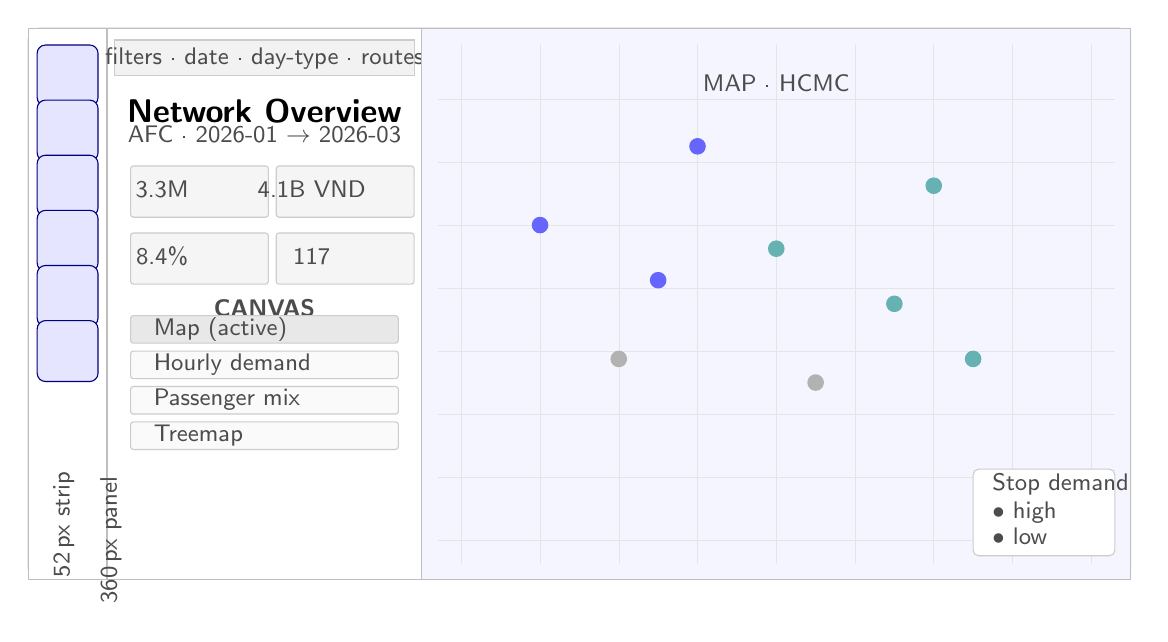
\begin{tikzpicture}[
    box/.style       ={rectangle, rounded corners=2pt,
                        font=\footnotesize\sffamily, align=center,
                        inner sep=4pt},
    icon/.style      ={rectangle, rounded corners=3pt,
                        draw=blue!50!black, fill=blue!10,
                        font=\small, minimum width=22pt,
                        minimum height=22pt, align=center},
    label/.style     ={font=\scriptsize\sffamily, color=gray!60!black},
]

\draw[draw=gray!50, rounded corners=4pt, fill=gray!2]
    (0,0) rectangle (14, 7);

% --- Icon strip ---
\draw[draw=gray!50, fill=white]
    (0,0) rectangle (1, 7);
\foreach \i in {0,1,2,3,4,5} {
    \node[icon] at (0.5, 6.4 - \i*0.7) {};
}
\node[label, rotate=90] at (0.45, 0.7) {52\,px strip};

% --- Analysis panel ---
\draw[draw=gray!50, fill=white]
    (1,0) rectangle (5, 7);

% Filter bar
\draw[draw=gray!40, fill=gray!10]
    (1.1, 6.4) rectangle (4.9, 6.85);
\node[label] at (3, 6.62) {filters · date · day-type · routes};

% Header
\node[box, font=\small\sffamily\bfseries] at (3, 5.95) {Network Overview};
\node[label] at (3, 5.65) {AFC · 2026-01 \(\rightarrow\) 2026-03};

% KPI grid
\foreach \r in {0,1} {
    \foreach \c in {0,1} {
        \draw[draw=gray!40, fill=gray!8, rounded corners=1pt]
            (1.3 + \c*1.85, 4.6 - \r*0.85) rectangle (3.05 + \c*1.85, 5.25 - \r*0.85);
    }
}
\node[label] at (1.7, 4.95) {3.3M};
\node[label] at (3.6, 4.95) {4.1B VND};
\node[label] at (1.7, 4.10) {8.4\%};
\node[label] at (3.6, 4.10) {117};

% Canvas selector
\node[label, font=\scriptsize\sffamily\bfseries] at (3, 3.45) {CANVAS};
\draw[draw=gray!40, fill=gray!18, rounded corners=1pt]
    (1.3, 3.0) rectangle (4.7, 3.35);
\node[label, anchor=west] at (1.45, 3.18) {Map (active)};
\foreach \i/\name in {1/Hourly demand, 2/Passenger mix, 3/Treemap} {
    \draw[draw=gray!40, fill=gray!4, rounded corners=1pt]
        (1.3, 3.0 - \i*0.45) rectangle (4.7, 3.35 - \i*0.45);
    \node[label, anchor=west] at (1.45, 3.18 - \i*0.45) {\name};
}

\node[label, rotate=90] at (1.05, 0.5) {360\,px panel};

% --- Canvas (map area) ---
\draw[draw=gray!50, fill=blue!4]
    (5,0) rectangle (14, 7);

\foreach \x in {5.5, 6.5, ..., 13.5}
    \draw[gray!20, very thin] (\x, 0.2) -- (\x, 6.8);
\foreach \y in {0.5, 1.3, ..., 6.5}
    \draw[gray!20, very thin] (5.2, \y) -- (13.8, \y);

\foreach \x/\y/\c in {6.5/4.5/blue, 8.0/3.8/blue, 9.5/4.2/teal,
                      11.0/3.5/teal, 7.5/2.8/gray, 10.0/2.5/gray,
                      12.0/2.8/teal, 8.5/5.5/blue, 11.5/5.0/teal} {
    \fill[\c!60] (\x, \y) circle (3pt);
}

\node[label] at (9.5, 6.3) {MAP · HCMC};

% Legend
\draw[draw=gray!40, fill=white, rounded corners=2pt]
    (12.0, 0.3) rectangle (13.8, 1.4);
\node[label, anchor=west] at (12.1, 1.20) {Stop demand};
\node[label, anchor=west] at (12.1, 0.85) {\(\bullet\)~high};
\node[label, anchor=west] at (12.1, 0.55) {\(\bullet\)~low};

\end{tikzpicture}
\caption{Three-column dashboard layout. The icon strip (52~px)
switches lenses; the analysis panel (360~px) holds filters, the
KPI grid and the canvas selector; the canvas (remainder of the
viewport) renders either the map or a single chart at a time.}
\label{fig:proposed:layout}
\end{figure}

Two binding rules govern the canvas: at most one chart is shown
at any time, and that chart fills at least 60\% of the viewport.
Liu's MCV literature~\cite{liu2022} shows that dense panels
crowded with small charts are a common failure mode of analytical
dashboards; Knaflic adds that an analyst's attention should be
directed to one analytical claim at a time~\cite{knaflic2015}.
The canvas-swap pattern enforces both: the panel renders no
charts of its own (only KPIs, lists, and selectors), and the
canvas renders one chart at canvas size --- typically 1500\,px
wide on a 1920\,px display.

\begin{figure}[H]
\centering
\includegraphics[width=0.95\linewidth]{images/screenshots/dashboard_network}
\caption{Dashboard with the Network Overview lens active and
the geospatial canvas in the default state. The icon strip is
on the far left; the analysis panel (filters, KPIs, canvas
selector, top-routes list) occupies the centre column; the
canvas occupies the remainder of the viewport.}
\label{fig:proposed:screenshot:network}
\end{figure}

\begin{figure}[H]
\centering
\includegraphics[width=0.95\linewidth]{images/screenshots/dashboard_route}
\caption{Dashboard with the Route Explorer lens active and
the QoS-2 distribution chart selected as the canvas. The map
returns one click away. Note that the panel itself contains
no charts --- only the lens-specific KPIs and the canvas
selector.}
\label{fig:proposed:screenshot:route}
\end{figure}

\subsection{Chart catalogue per lens}

Table~\ref{tab:proposed:charts} lists the chart that each canvas
option produces, alongside the analytical question it answers and
the literature primitive (where applicable) that grounds the
visualisation choice.

\begin{table}[H]
\centering
\caption{Chart catalogue. Each row is one canvas option in the
dashboard.}
\label{tab:proposed:charts}
\renewcommand{\arraystretch}{1.20}
\begin{tabularx}{\linewidth}{p{2.0cm}p{3.4cm}p{3.0cm}X}
\hline
\textbf{Lens} & \textbf{Canvas} & \textbf{Chart type} & \textbf{Question} \\
\hline
Network       & Hourly demand          & Stacked area, AM/PM bands & When does demand peak? \\
Network       & Passenger mix          & Donut, four segments      & Who rides? \\
Network       & Demand pattern cluster & Heatmap, GroupSet groups~\cite{liu2022} & Which routes share a daily shape? \\
Network       & Route health treemap   & Treemap, ghost-rate colour & Which routes underperform? \\
Network       & Operator scatter       & Bubble scatter            & How do companies compare? \\
\hline
Route         & Hourly demand          & Stacked area              & When is this route busy? \\
Route         & QoS-1 trend            & Daily line~\cite{srisakaokul2023} & Are scheduled trips actually running? \\
Route         & QoS-2 distribution     & Histogram~\cite{srisakaokul2023}  & How on-route are GPS trajectories? \\
Route         & QoS-3 box plot         & Per-stop box~\cite{srisakaokul2023} & Where on the route does delay accumulate? \\
Route         & Speed corridor         & Map polyline + FuzzyCut~\cite{liu2022} & Where is this route slow? \\
Route         & Trip Gantt             & Gantt, anomaly highlight  & How do trips line up across the day? \\
Route         & Tet vs.\ normal        & Side-by-side line         & How did Tet affect demand? \\
\hline
Stop          & Hourly demand          & Bar chart                 & When is this stop busy? \\
Stop          & Routes $\times$ hour   & Heatmap                   & Which routes feed this stop and when? \\
Stop          & Multi-stop comparison  & Radar, 2--4 stops         & How do these stops compare? \\
Stop          & Spatial accessibility  & Grid choropleth, Gridify~\cite{liu2022} & Which areas are underserved? \\
\hline
Financial     & Daily revenue          & Bar, weekday/weekend      & When does the network earn revenue? \\
Financial     & Payment channels       & Horizontal bar, \% labels & How do passengers pay? \\
Financial     & Worst ghost-rate routes& Ranked horizontal bar     & Which routes waste fuel? \\
Financial     & Revenue scatter        & Bubble scatter            & Who earns vs.\ who is subsidised? \\
Financial     & Revenue efficiency     & Histogram + FuzzyCut~\cite{liu2022} & How do we band routes by revenue? \\
\hline
Metro         & Feeder catchment       & Concentric rings on map   & How well do buses feed the metro? \\
\hline
\end{tabularx}
\end{table}

The chart-type column is deliberately conservative: stacked area
charts for time series, histograms for distributions, scatter
plots for two-variable relationships, treemap for hierarchical
size $+$ colour encoding. Knaflic argues that the analyst's
attention should be on the data and the analytical claim, not on
the novelty of the chart~\cite{knaflic2015}; the dashboard
therefore prefers the canonical chart type for each question over
a more ornate alternative.

\subsection{Cross-lens interactions}

The MCV interaction model (Section~\ref{sec:theory:mcv}) connects
the lenses into a coherent dashboard. Three cross-lens
interactions are particularly relevant in practice.

\paragraph{Treemap tile $\rightarrow$ Route Explorer.}
A click on any tile in the Network route-health treemap sets the
\texttt{selected\_route} field in the shared session-state object
and switches the active lens to Route Explorer. The filter bar is
preserved, so the analyst arrives at the route-level view already
narrowed to the date range, day type, and hour band that were
active in the treemap.

\paragraph{Map stop $\rightarrow$ Stop Analysis.}
A click on any stop on the geospatial canvas sets
\texttt{selected\_stop\_key} and switches to Stop Analysis. The
panel re-populates with the boardings, dwell, and per-route
breakdown for the chosen stop, again preserving the global
filter context.

\begin{figure}[H]
\centering
\includegraphics[width=0.95\linewidth]{images/screenshots/dashboard_stop}
\caption{Stop Analysis lens reached by clicking a stop on the
geospatial canvas. The selected stop's boardings, peak hour,
average fare, and routes-served list populate the panel without
any explicit filter change by the analyst.}
\label{fig:proposed:screenshot:stop}
\end{figure}

\paragraph{Worst-ghost ranking $\rightarrow$ Route Explorer
$+$ ghost-only filter.} A click on a route in the Financial
worst-ghost ranking switches to Route Explorer with the route
selected and an additional filter applied that scopes the canvas
to only the trips classified as near-ghost. This is the
``drill-from-symptom-to-cause'' pattern advocated by
Knaflic~\cite{knaflic2015}: the analyst sees an anomaly in
aggregate, clicks once, and lands at the trip-level view that
explains it.


% ============================================================
% Chapter 4 — Current Prototype (NEW, advisor-requested)
% ============================================================
\chapter{Current Prototype}
\label{chapter:prototype}

\textit{This chapter presents the artefacts produced during
Phase~1: the exploratory analysis on which the solution is
grounded, the high-fidelity UI mockup that locks the dashboard's
visual language, the data-pipeline skeleton that already executes
against the local sample, and the supporting design artefacts.}

\section{Exploratory Analysis Findings}
\label{sec:prototype:eda}

The exploratory data analysis is captured in four executed
Jupyter notebooks~\cite{jupyter} in the project's
\texttt{notebooks/} directory. The notebooks are the empirical
ground truth on which every design decision in
Chapter~\ref{chapter:proposed} rests; each notebook is executed
via \texttt{jupyter nbconvert --execute --inplace} and committed
with its rendered outputs embedded, so report figures can
reference notebook cells directly.

\paragraph{Notebook 01 --- Schema and volume.}
Surveys the parquet exports produced by
\texttt{src/duckdb\_loader.py} and reports the two headline
volume figures that bound the design space: 17{,}883{,}623 AFC
boarding events over the ninety-day window
(2026-01-01 to 2026-03-31), and 720{,}088 GPS pings for the
local one-day sample (2025-03-18). The notebook also verifies
the cross-source overlap (one hundred and twenty-one of one
hundred and sixty-three routes appear in both sources) which
grounds the GPS$\leftrightarrow$AFC reconciliation rule in
\texttt{dim\_route} (Section~\ref{sec:proposed:warehouse_local}).

\paragraph{Notebook 02 --- GPS-side analysis.}
Profiles the local one-day GPS sample. Confirms the
extracted-trips buffer contains nine routes (29, 41, 57, 61, 84,
99, 102, 141, 151), enumerates the one hundred and thirty-one
distinct vehicles, and sanity-checks the door-up and door-down
sensor fields that underpin the ghost-stop and ghost-run
detection planned for the Spatial and Financial cards.

\paragraph{Notebook 03 --- AFC fare and revenue analysis.}
Produces the most consequential finding of the EDA: thirty-four
percent of all boardings on weekday mornings use a student-fare
ticket (6{,}162{,}862 HS-SV tickets out of the 17.8~million
total), and 96.2\% of payments are cash-equivalent. The notebook
identifies the eight universities that anchor the student-fare
share (HCMUS, HCMUT, UEH, GTVT, USSH, HCMUTE, UIT, SGU),
computes the quarterly revenue of approximately
\textcent~72.4~billion, and detects the visible T\d ết dip from
28~January to 5~February 2026.

\paragraph{Notebook 04 --- Stops, schools, and metro.}
Documents the 4{,}710 stops with verified latitude/longitude
and the nineteen metro feeder routes referenced in the dataset
specification~\cite{hcmcgps2025}. Identifies the gap in school
geocoding (the sixty-four school addresses arrive without
coordinates, so \texttt{dim\_school} ships with district-level
stubs initially) and the schedule-data anomaly of ninety-one
thousand \texttt{service\_type=`unknown'} rows that requires
cleaning before any adherence-related chart can render.

\begin{figure}[H]
\centering
\imageplaceholder{Chart (Calendar heatmap)}{A calendar heatmap
of student-fare boardings over the 90-day AFC window, rows =
weeks, columns = days-of-week, colour = student-fare boarding
count. The morning-peak compression on weekdays is the visible
finding; the T\d ết flatline (28~January--5~February) is the
secondary finding. Generated from notebook 03.}{Run
\texttt{notebooks/03\_fare\_revenue.ipynb} cell labelled
``student fare weekly heatmap''. Export the resulting plotly
figure as PNG at $\geq$1200~px wide. Save as
\texttt{images/screenshots/eda\_student\_fare\_calendar.png}.}
\caption{Student-fare boardings by date and weekday, from
Notebook~03. The morning-peak compression on weekdays is the
empirical basis for the flagship card
(Section~\ref{sec:proposed:sdvf}); the T\d ết flatline is the
natural-experiment window for Anomaly Lab Chart~5.5.}
\label{fig:prototype:eda_student_fare}
\end{figure}

The five EDA findings that drove design decisions are documented
in Section~\ref{sec:proposed:eda_to_design}; this section
documents the artefacts (the notebooks themselves) that
\emph{produced} those findings, satisfying the Phase~1
deliverable ``Phát triển, thử nghiệm và đánh giá ban đầu''
required by the capstone topic description~\cite{capstoneDescription}.

\section{Interactive Mockup}
\label{sec:prototype:mockups}

The dashboard's visual language is locked in a single-file
high-fidelity HTML mockup published at
\texttt{docs/design/app-layouts.html}. The mockup is not a
Streamlit prototype but a pixel-accurate reference that the
Streamlit implementation will reproduce in Phase~2 through a
combination of native Plotly charts (twenty-two of thirty-one
charts), native pydeck maps (six charts), and embedded HTML
components for the hub itself plus the three custom chart types
(Marey, GroupSet/UpSet, scrollytelling Stories).

\begin{figure}[H]
\centering
\imageplaceholder{Screenshot}{The hub mockup, vertical
editorial scroll. Six alternating cards each with a unique
accent colour (orange / gold-flagship / green / red / purple /
slate), a teaser SVG matching the card's principal chart type,
and a story-subtitle pull-quote. Date-range pill ``Jan~1--Mar~31,
2026'' in the top bar; ``Cards $\downarrow$'' and ``Stories
$\downarrow$'' dropdown menus.}{Open
\texttt{docs/design/app-layouts.html} in a browser at 1280~px
width; take a full-page screenshot covering the entire hub
section. Save as
\texttt{images/screenshots/hub\_v8\_full.png}.}
\caption{The hub mockup: six alternating cards with per-card
accent colours and chart-type teasers (Section~\ref{sec:proposed:hub}).}
\label{fig:prototype:hub}
\end{figure}

\begin{figure}[H]
\centering
\imageplaceholder{Screenshot}{The card-interior mockup for
Card~2 (Demand \& Crowding), Route $\times$ Hour heatmap
active. The 108-pixel rail on the left lists the five charts in
the theme; the filter bar above the canvas carries the
per-chart filter chips and a breadcrumb; the canvas is a
heatmap with a click pop-up open over one cell.}{Scroll to the
second mockup section in
\texttt{docs/design/app-layouts.html}. Take a screenshot of the
card interior with a pop-up active. Save as
\texttt{images/screenshots/card\_interior\_demand.png}.}
\caption{The card interior: a narrow rail of chart options on
the left, a single big-canvas chart on the right with a
per-chart filter bar, a click pop-up demonstrating the A1
linked-brushing invariant (Section~\ref{sec:proposed:card}).}
\label{fig:prototype:card}
\end{figure}

\begin{figure}[H]
\centering
\imageplaceholder{Screenshot}{The A3 universal entity-detail
panel, shown for Route~152. Side panel covers approximately
forty percent of the viewport on the right, with tabs
``Overview'', ``Demand'', ``Reliability'', ``Network'',
``Context''. Shows a KPI strip, a small spark-line history, a
``Routes like this one'' card with three UMAP neighbours, and a
drill-down action list.}{Scroll to the entity-panel section in
\texttt{docs/design/app-layouts.html}; take a screenshot
covering the panel and the chart canvas it overlays. Save as
\texttt{images/screenshots/entity\_panel.png}.}
\caption{The A3 universal entity-detail panel, opened on a
route click (Section~\ref{sec:proposed:invariants}).}
\label{fig:prototype:panel}
\end{figure}

The mockup also documents the cross-card navigation drop-downs
in the top bar, the hover-tooltip glossary for technical terms
(QoS-1/2/3, AFC, Marey, UMAP, etc.), and the four scrollytelling
Stories that run as a separate section of the hub
(Section~\ref{sec:proposed:stories}). The published mockup is
the artefactual evidence of the dashboard specification in
Chapter~\ref{chapter:proposed}; locking it before any Streamlit
code is written is the Phase~1 deliverable that lets Phase~2
proceed without further visual-design work.

\section{Data-Pipeline Skeleton}
\label{sec:prototype:warehouse}

The warehouse described in
Section~\ref{sec:proposed:warehouse_local} is implemented to
Layer~1 (raw views) in
\texttt{src/duckdb\_loader.py}~\cite{duckdb}. The module exposes
a single class \texttt{BusDuckDB} whose \texttt{normalize()}
method converts the upstream CSV exports to ZSTD-compressed
parquet under \texttt{data/parquet/}, and whose
\texttt{register\_views()} method registers the twenty-four raw
views that Layer~2 dimensions will read from in Phase~2. The
class is exercised through direct execution against the local
sample (one day of GPS, ninety days of AFC) and feeds the four
EDA notebooks (Section~\ref{sec:prototype:eda}).

\begin{table}[H]
\centering
\caption{Layer~1 raw views registered by
\texttt{src/duckdb\_loader.py}.}
\label{tab:prototype:rawviews}
\footnotesize
\renewcommand{\arraystretch}{1.15}
\begin{tabularx}{\linewidth}{p{3.4cm}X}
\hline
\textbf{Domain} & \textbf{Views} \\
\hline
GPS (operations) &
\texttt{gps\_raw}, \texttt{gps\_trips}, \texttt{gps\_stop\_times},
\texttt{gps\_schedules}, \texttt{gps\_routes},
\texttt{gps\_companies}, \texttt{gps\_vehicles},
\texttt{gps\_drivers}, \texttt{gps\_stations},
\texttt{gps\_extracted} \\
AFC (demand) &
\texttt{tickets}, \texttt{payments}, \texttt{ticket\_trips},
\texttt{ticket\_routes}, \texttt{ticket\_companies},
\texttt{ticket\_buses}, \texttt{ticket\_stations},
\texttt{ticket\_route\_stops}, \texttt{ticket\_drivers},
\texttt{ticket\_users}, \texttt{ticket\_students},
\texttt{ticket\_schools} \\
Shared & \texttt{stops}, \texttt{mapping} \\
\hline
\end{tabularx}
\end{table}

Layers~2--4 of the warehouse (conformed dimensions, fact views,
aggregate tables) are Phase~2 deliverables, scheduled in
Section~\ref{sec:future:roadmap} and detailed in
Appendix~\ref{appendix:plan}. The Phase~1 commitment is that
the Layer~1 views, the schema diagram of
Section~\ref{sec:proposed:dataarch}, and the chart-to-aggregate
data contract of Section~\ref{sec:proposed:modules} together
form a sufficient specification for Phase~2 implementation to
follow without further design work.

The warehouse is designed to persist on disk at
\texttt{db/bus.duckdb}, so that app cold-start time in Phase~2
is bounded by view registration (sub-second) rather than CSV
normalisation (approximately thirty seconds for the local
sample; approximately five minutes for the full fifty-day GPS
dataset). The DataFrame layer uses Polars~\cite{polars} where
column-major performance matters and pandas elsewhere; the
forecasting work of Chart~2.5 uses
statsforecast~\cite{statsforecast}; the dimensionality reduction
of Chart~6.1 uses UMAP~\cite{umap}; the hex-grid aggregation of
Chart~3.2 uses Uber's H3~\cite{h3}; the Streamlit
shell~\cite{streamlit} reads Layer~4 aggregates through
\texttt{@st.cache\_data}; charts render through
Plotly~\cite{plotly} and pydeck~\cite{pydeck} with embedded HTML
components via \texttt{st.components.v1.html} where Plotly does
not natively support the chart type.

\section{Design Artefacts}
\label{sec:prototype:artifacts}

\noindent\textit{Stub --- this section catalogues the durable
Phase~1 design artefacts (CLAUDE.md project log, the brainstorm
corpus) and explains their roles as the authoritative source of
truth for Phase~2 implementation. Content to be filled by
subagent~F4.}


% ============================================================
% Chapter 5 — Future Work (NEW, advisor-requested)
% ============================================================
\chapter{Future Work}
\label{chapter:future}

\textit{This chapter sketches the Phase~2 implementation roadmap,
the data activations that unlock currently-deferred features, the
predictive extensions that follow naturally from the historical
foundation laid in Phase~1, and the external integrations and
user-validation study that close the design loop.}

\section{Phase 2 Implementation Roadmap}
\label{sec:future:roadmap}

Phase~2 of this thesis is the implementation of the dashboard
specified in Chapter~\ref{chapter:proposed}. The work is
organised into nine phases, P1--P9, each producing a working
demoable artefact. The phases are summarised in
Table~\ref{tab:future:roadmap}; their critical path is
P1~$\rightarrow$~P2 and the remaining phases are largely
parallelisable. Per Câu~5 of the grading
rubric~\cite{rubric}, the plan covers content, time, personnel,
and expected outcomes; full per-phase deliverables and
acceptance criteria are tabulated in
Appendix~\ref{appendix:plan}.

\begin{table}[H]
\centering
\caption{Phase 2 implementation phases, deliverables, and
estimated effort.}
\label{tab:future:roadmap}
\footnotesize
\renewcommand{\arraystretch}{1.20}
\begin{tabularx}{\linewidth}{p{0.9cm}p{4.2cm}Xp{1.4cm}}
\hline
\textbf{Ph.} & \textbf{Deliverable} & \textbf{Outcome} & \textbf{Effort} \\
\hline
P1 & Warehouse Layers 2--4 build
   & \texttt{dim\_*}, \texttt{fact\_*}, three \texttt{agg\_*}
     tables; build CLI; validation notebook 05
   & 2~days \\
P2 & End-to-end Card~2 (Demand)
   & Five charts render; linked brushing across all five; A3
     entity panel for routes; cold-load $<$~3~s; warm render
     $<$~50~ms
   & 3~days \\
P3 & Spatial card + pydeck
   & Stop Demand Explorer, hex density grid, network overview;
     \texttt{agg\_stop\_hour} populated
   & 2~days \\
P4 & School flagship card
   & Schools $\rightarrow$ Routes treemap, school-routeness
     classifier, equity map (district stubs)
   & 2~days \\
P5 & Financial + Network Health cards
   & P\&L quadrant, operator scorecard, payment adoption,
     QoS-1/2/3 scorecard, anomaly threshold-$T$ slider
   & 3~days \\
P6 & Routes card with Marey
   & Discovery (UMAP, archetype) and Detail modes; embedded
     Marey and GroupSet HTML components
   & 3~days \\
P7 & Hub + entity-panel polish
   & Editorial hub HTML embedded; A3 panel for all six entity
     types; URL state; export
   & 2~days \\
P8 & Stories scrollytelling
   & Four scenes-driven stories with Scrollama; scene JSON
     authoring
   & 2~days \\
P9 & Final polish + evaluation
   & Verified school geocoding; full 50-day GPS loaded if
     available; perf tuning; screen recording; initial user
     evaluation
   & 2~days \\
\hline
\multicolumn{3}{r}{\textbf{Total estimated:}} & 21~days \\
\hline
\end{tabularx}
\end{table}

\begin{figure}[H]
\centering
\imageplaceholder{Diagram (Gantt chart)}{A horizontal Gantt
chart with nine bars labelled P1--P9, the x-axis covering days
0--21. P1 (days 0--2, blue), P2 (days 2--5, blue), P3 (days
5--7, green; can start after P1+P2), P4 (days 5--7, gold; can
parallel with P3), P5 (days 7--10, red), P6 (days 10--13,
purple), P7 (days 13--15, cyan), P8 (days 15--17, orange), P9
(days 17--21, grey). Dependency arrows: P1 $\rightarrow$ P2;
P2 $\rightarrow$ P3, P4; P3, P4 $\rightarrow$ P5;
P5 $\rightarrow$ P6; P6 $\rightarrow$ P7; P7 $\rightarrow$ P8;
P8 $\rightarrow$ P9.}{Draw in a tool such as
\texttt{draw.io}, \texttt{Lucidchart}, or \texttt{Excalidraw};
export as PNG at $\sim$300~DPI. Save as
\texttt{images/diagrams/phase2\_gantt.png}.}
\caption{Phase 2 Gantt: nine phases over approximately 21
days. P3 and P4 can run in parallel after P1+P2 complete.}
\label{fig:future:gantt}
\end{figure}

\paragraph{Content.}
The plan content is the nine phases above. Each phase produces
one or two artefacts that the next phase depends on; the
Appendix~\ref{appendix:plan} table records the exact acceptance
criterion per phase (e.g., for P1: the build CLI runs in
$<$~30~s on the local sample and emits eight aggregate tables).

\paragraph{Time.}
Total estimated effort is twenty-one working days at one
developer. The critical path is P1~$\rightarrow$~P2 (five
working days); the remaining sixteen days are parallelisable in
P3+P4 (the spatial and the school cards run independently
because their aggregate tables \texttt{agg\_stop\_hour} and
\texttt{agg\_school\_route} are independent) and otherwise
sequential.

\paragraph{Personnel.}
Phase~2 is single-author. Time tracking is per-phase rather
than per-task because every phase is small enough for one
developer to hold the full context. The thesis advisor reviews
at the end of P2 (first end-to-end card) and at the end of P6
(all cards rendering) before sign-off.

\paragraph{Expected outcomes.}
At the end of Phase~2, the dashboard renders thirty out of
thirty-one charts at sub-fifty-millisecond warm latency;
supports linked brushing within every card and the universal
entity-detail panel (A3 of
Section~\ref{sec:proposed:invariants}) on every clickable
element; persists state to a shareable URL; and exports every
chart as PNG/PDF/CSV with a single click. The final chart, the
Marey time--distance diagram, depends on the full GPS pull
(Section~\ref{sec:future:gps}) and is delivered at the start
of P9 if the data is available, or deferred to a follow-on
phase if not.

\paragraph{Risk and mitigation.}
Four risks dominate the schedule. (1)~Streamlit performance
falling below the budget
(Section~\ref{sec:proposed:problem}); the mitigation is to fall
back to embedded HTML components for hot paths, which is
already the case for three charts. (2)~The full GPS pull from
Kaggle failing or taking longer than expected; the mitigation
is to demo with the local one-day sample and document the
seven charts that remain at SHOULD/WON'T tier until the pull
completes. (3)~School geocoding under target before P9
deadline; the mitigation is to ship the dashboard with
district-level approximation and the
``verified~\checkmark'' badge described in
Section~\ref{sec:proposed:warehouse_local}.
(4)~Linked-brushing latency feeling sluggish on Streamlit's
server-side rerun model; the mitigation is to pre-compute the
highlight sets server-side so only the chart's colour column
is recomputed on rerun, not the data itself.

\section{Full GPS Dataset Activation}
\label{sec:future:gps}

\noindent\textit{Stub --- this section enumerates the seven
charts unlocked once the full fifty-day GPS dataset is loaded.
Content to be filled by subagent~G2.}

\section{Predictive Extensions}
\label{sec:future:predictive}

\noindent\textit{Stub --- this section sketches three
predictive extensions: arrival-time prediction (Lin~\&~Zeng),
per-route anomaly detection, and the bus-as-traffic-sensor map
(Derevitskiy). Content to be filled by subagent~G3.}

\section{External Integrations and User Validation}
\label{sec:future:external}

Two further lines of work close the Future Work chapter.

\paragraph{The ``Ask the Data'' natural-language interface.}
A separate external team is developing a natural-language query
interface that translates a question typed in plain English or
Vietnamese (``Which route had the most ghost trips in March?'')
into DuckDB SQL and renders the answer as a chart. Integrating
the interface into the dashboard requires no architectural
change beyond exposing the eight aggregate tables and three
fact views as a query target; the integration is planned as a
seventh hub card (\emph{Ask the Data}, shown as the
``UPCOMING'' card in the hub mockup of
Section~\ref{sec:prototype:mockups}).

\paragraph{User validation study.}
The capstone topic description~\cite{capstoneDescription} names
``Đánh giá và cải tiến'' (evaluation and improvement) as a
Phase~2 task. The plan is a formal user study with three or
four members of each of the four user roles
(Section~\ref{sec:proposed:problem}): MCPT operators,
bus-company analysts, student commuters, and new bus users.
The study measures two outcomes: the operators' ability to
answer their canonical questions using the dashboard, and the
discovery of analytical questions that the dashboard can
answer but that the stakeholders had not previously
articulated. The study is scheduled for after P9 completion
(Section~\ref{sec:future:roadmap}) and is documented as a
deliverable in Appendix~\ref{appendix:plan}.

\paragraph{Closing.}
Together with the Phase~2 roadmap of
Section~\ref{sec:future:roadmap}, the data activations of
Section~\ref{sec:future:gps}, and the predictive extensions of
Section~\ref{sec:future:predictive}, the present chapter
covers Câu~5 of the grading rubric~\cite{rubric} in full ---
\emph{nội dung, thời gian, nhân sự, và kết quả mong đợi}
(content, time, personnel, and expected outcomes).


% ============================================================
% Chapter 6 — Conclusion (Contributions section lives here per advisor's note)
% ============================================================
\chapter{Conclusion}
\label{chapter:conclusion}

\section{Summary}
\label{sec:conclusion:summary}

This Phase~1 report has presented the design of \textbf{BusLens},
a visual analytics platform for the Ho Chi Minh City public bus
network. Chapter~\ref{chapter:intro} motivated the work as the
engineering response to the absence of any analytical tool over
the network's three large data streams (raw GPS pings, AFC
ticketing events, and static GTFS metadata).
Chapter~\ref{chapter:background} surveyed four bodies of prior
work --- bus operational analytics (Srisakaokul, Derevitskiy,
Lin~\&~Zeng), visualisation of spatial-temporal traffic data
(Liu), bus--metro intermodal connectivity, and existing HCMC
tooling --- and developed the theoretical foundations of the
solution: the four-layer warehouse adapted from the medallion
pattern~\cite{databricksMedallion}, the analytical-stack choice
(DuckDB~\cite{duckdb} + Streamlit~\cite{streamlit} +
Plotly~\cite{plotly} + pydeck~\cite{pydeck} +
\texttt{st.components.v1.html}), the QoS scoring
framework~\cite{srisakaokul2023}, the visualisation primitives
of Liu~\cite{liu2022} plus the Marey time--distance
diagram~\cite{linzeng2014}, the visual-storytelling principles
of Knaflic~\cite{knaflic2015}, and the Multiple Coordinated
Views interaction model that the dashboard's linked-brushing
invariant implements.

Chapter~\ref{chapter:proposed} developed the proposed solution
along six axes: a formal problem statement; an SDVF tier
prioritisation; a four-layer warehouse design with eight
aggregate tables that compose a hard data contract with the
chart catalogue; the EDA findings that scope every downstream
decision; a thirty-one chart catalogue with chart-to-aggregate
mapping and SDVF tiers; and the dashboard's
Hub~$\rightarrow$~Card~$\rightarrow$~Chart information
architecture with the A1, A2, A3 behavioural invariants and the
Stories scrollytelling layer.
Chapter~\ref{chapter:prototype} documented the four executable
deliverables of Phase~1: the EDA notebooks, the UI mockup, the
warehouse skeleton, and the supporting design artefacts.
Chapter~\ref{chapter:future} sketched the Phase~2
implementation roadmap, the data activations that unlock the
deferred charts, and the predictive extensions and external
integrations that follow the historical foundation.

\section{Achievements}
\label{sec:conclusion:achievements}

Three achievements of this Phase~1 work deserve emphasis.

\paragraph{A unified data foundation.}
The four-layer warehouse design reconciles three previously
siloed data streams behind a single SQL surface, with
reproducible normalisation from the upstream parquet exports
and consistent type-casting in
\texttt{src/duckdb\_loader.py}. The foundation is reusable for
any future analytical work on the same data, including the
natural-language ``Ask the Data'' interface under development
by another team
(Section~\ref{sec:future:external}).

\paragraph{A research-grounded analytics suite.}
Each visualisation primitive used in the dashboard traces back
to a specific peer-reviewed source. The QoS-1/2/3 scoring
framework of Srisakaokul~\textit{et~al.}~\cite{srisakaokul2023},
originally delivered as an offline study, is wired into an
interactive tool. The FuzzyCut, GroupSet, and Gridify primitives
of Liu~\cite{liu2022}, originally demonstrated on highway-sensor
and taxi data, are transferred to the urban-bus operational
domain. The Marey time--distance
diagram~\cite{linzeng2014} is the principal Detail-mode chart
of the Routes card. The MCV interaction model is implemented at
full scope across the dashboard as the A1 invariant. The
result is a tool whose every analytical claim is grounded in a
citable source.

\paragraph{A unified, role-anchored interactive interface.}
The Hub~$\rightarrow$~Card~$\rightarrow$~Chart hierarchy, the
single-chart canvas rule, the three A1/A2/A3 behavioural
invariants, and the shared session-state object together
deliver a dashboard specification that scales from a
1366$\times$768 laptop screen to a defence-room projector and
serves four distinct user roles (passenger, driver, company,
MCPT) from a single chrome without forcing any of them to leave
the analytical context their question begins in.

\section{Limitations}
\label{sec:conclusion:limitations}

The work has four limitations that should be acknowledged.

\paragraph{Single-day GPS sample.}
The local GPS dataset covers a single day (2025-03-18) over
nine routes. The full fifty-day dataset is referenced in the
dataset specification~\cite{hcmcgps2025} and is reachable but
not loaded locally. Seven charts in the catalogue
(Section~\ref{sec:proposed:milestones}) remain at SHOULD or
WON'T-tier until the full dataset is loaded; the activation is
scheduled at the start of P9
(Section~\ref{sec:future:gps}).

\paragraph{Calendar mismatch between GPS and AFC.}
GPS data spans March 2025 while AFC tickets span
January--March 2026. The two streams cannot be joined by
timestamp and are treated as complementary sources whose
findings are combined narratively in the dashboard at the
\texttt{route}~$\times$~\texttt{hour-of-day}~$\times$~\texttt{day-type}
aggregate grain (Section~\ref{sec:proposed:schema}). A future
data release that produces overlapping GPS and AFC windows
would let the cross-source analysis happen at finer grains.

\paragraph{No alighting data.}
AFC records boarding events only. ``Passengers on the bus at
time~$T$'' is therefore not a directly computable quantity;
all crowding analyses are framed in terms of boardings per
stop or per trip. The limitation is documented visibly in the
Stop Demand Explorer (Chart~3.3) and the Network Health card
so end users encounter it before forming unrealistic
expectations.

\paragraph{QoS-2 sensitivity to GPS noise.}
In the dense urban canyons of HCMC, GPS positioning noise
causes pings to fall outside the 50-metre route buffer even
when the bus is in fact on-route. This systematically lowers
absolute QoS-2 scores; the metric is therefore safer to
interpret relatively (comparing routes to each other) than
absolutely. The Reliability scorecard (Chart~5.4) will surface
this caveat as an informational callout next to the QoS-2 KPI.

\section{Contributions}
\label{sec:conclusion:contributions}

Per the advisor's instruction, the contributions of this work
are summarised at the end of the report so that the reader
encounters them after the evidence rather than before.
Phase~1 of this thesis focuses on solutioning and prototyping;
the contributions are therefore deliberately scoped and short.

\paragraph{1. A reconciled design specification.}
Two parallel data streams (GPS and AFC) and four stakeholder
groups (passenger, driver, company, MCPT operator) are
reconciled into a single dashboard specification of six themed
cards and thirty-one canonical charts, with explicit invariants
for linked brushing, story-subtitled charts, and a universal
entity detail panel
(Chapters~\ref{chapter:proposed} and~\ref{chapter:prototype}).

\paragraph{2. A four-layer warehouse design.}
A four-layer DuckDB warehouse design (raw views, conformed
dimensions, fact views, pre-computed aggregate tables) is
specified, partially scaffolded (Layer~1), and justified
against two design alternatives. Each of the thirty-one charts
in the design is mapped to exactly one of eight aggregate views
as a hard data contract
(Sections~\ref{sec:proposed:warehouse_local}
and~\ref{sec:proposed:modules}).

\paragraph{3. An evidence-grounded module scoping.}
Four executed Jupyter notebooks (\texttt{notebooks/01--04})
produce the eleven headline EDA findings on which the SDVF
tier prioritisation is grounded, including the thirty-four
percent student-fare share that anchors the flagship card and
the calendar mismatch that forces a row-level join between GPS
and AFC to be ruled out
(Chapter~\ref{chapter:prototype}).

\paragraph{4. A high-fidelity, role-anchored UI mockup.}
A pixel-accurate light-theme mockup of the hub, one card
interior, and the universal entity-detail panel is published
at \texttt{docs/design/app-layouts.html}, locking the visual
language before any Streamlit code is written
(Section~\ref{sec:prototype:mockups}).

\paragraph{Mapping to the capstone topic deliverables.}
The capstone topic description~\cite{capstoneDescription}
names five Phase~1 tasks. Their coverage in this report is:
\emph{(i)~studying the HCMC bus dataset} →
Section~\ref{sec:prototype:eda};
\emph{(ii)~proposing analytical problems} →
Sections~\ref{sec:proposed:problem}
and~\ref{sec:proposed:modules};
\emph{(iii)~designing the analysis and visualisation
solution} → Chapters~\ref{chapter:proposed}
and~\ref{chapter:prototype};
\emph{(iv)~researching and selecting techniques and tools} →
Chapter~\ref{chapter:background} and the alternatives-considered
subsections~\ref{sec:proposed:warehouse_alts},
\ref{sec:proposed:module_rationale},
\ref{sec:proposed:dashboard_alts};
\emph{(v)~developing, testing, and conducting initial
evaluation} → partially met by the warehouse skeleton
(Section~\ref{sec:prototype:warehouse}) and the executed
notebooks (Section~\ref{sec:prototype:eda}); full Phase~2
development continues per the roadmap of
Chapter~\ref{chapter:future}.

A formal implementation and user study are out of scope for
Phase~1 and are sketched in Chapter~\ref{chapter:future}.


\renewcommand{\bibname}{References}
\addcontentsline{toc}{chapter}{References}
\printbibliography

\appendix

\chapter*{Appendix A --- Warehouse DDL Excerpts}
\label{appendix:ddl}
\addcontentsline{toc}{chapter}{Appendix A --- Warehouse DDL Excerpts}

\noindent\textit{Stub --- this appendix shows the DDL of the
four key warehouse tables (\texttt{dim\_route},
\texttt{dim\_date}, \texttt{fact\_boardings},
\texttt{agg\_route\_hour}). Content to be filled by
subagent~I2.}

\chapter*{Appendix B --- Phase 2 Plan}
\label{appendix:plan}
\addcontentsline{toc}{chapter}{Appendix B --- Phase 2 Plan}

This appendix details the Phase~2 plan in full, complementing the
narrative roadmap of Section~\ref{sec:future:roadmap}. Together,
the chapter and the appendix address Câu~5 of the grading
rubric~\cite{rubric} on all four dimensions: content, time,
personnel, and expected outcomes.

\section*{B.1 Deliverables per phase}

Each phase produces one or more deliverables that the next
phase depends on. The acceptance criterion for each phase is
the boolean condition under which that phase is considered
complete and the next phase can begin.

\begin{table}[H]
\centering
\caption{Phase 2 deliverables, expected outcomes, and acceptance
criteria.}
\label{tab:appendix:deliverables}
\footnotesize
\renewcommand{\arraystretch}{1.2}
\begin{tabularx}{\linewidth}{p{0.7cm}p{3.6cm}X}
\hline
\textbf{Ph.} & \textbf{Deliverable} & \textbf{Acceptance criterion} \\
\hline
P1 & Warehouse Layers 2--4 build
   & \texttt{python -m src.warehouse.builder} runs in
     $<$~30~s on local sample and emits ten \texttt{dim\_*}
     tables, three \texttt{fact\_*} views, and eight
     \texttt{agg\_*} tables; \texttt{notebook 05} asserts row
     counts match facts. \\
P2 & End-to-end Card~2 (Demand)
   & All five charts render; linked brushing works across all
     five; A3 entity panel opens on any route click; cold-load
     $<$~3~s; warm render $<$~50~ms. \\
P3 & Spatial card + pydeck
   & H3 hex layer renders at three cell sizes; Stop Demand
     Explorer renders 4{,}710 stops without UI lag. \\
P4 & School flagship card
   & Schools $\rightarrow$ Routes treemap renders;
     school-routeness classifier renders for all 163 routes;
     equity map renders at district resolution. \\
P5 & Financial + Network Health cards
   & P\&L quadrant clickable; QoS-1/2/3 scores computed on the
     nine routes available in the local GPS sample;
     threshold-$T$ slider snaps between the five pre-computed
     levels. \\
P6 & Routes card with Marey
   & Discovery and Detail modes both render; Marey diagram is
     interactive (zoom, hover trip); GroupSet matrix shows the
     four archetypes correctly. \\
P7 & Hub + entity-panel polish
   & Hub HTML renders inside Streamlit with no layout
     breakage; the A3 panel works for all six entity types;
     URL state survives a browser refresh. \\
P8 & Stories scrollytelling
   & All four stories scroll-driven; each scene deep-links into
     the matching card view; reading-progress bar visible. \\
P9 & Final polish + evaluation
   & School geocoding verified for $\geq$~50 of 64 schools;
     full 50-day GPS loaded if available; two-minute
     screen-recording demo produced; initial user evaluation
     with $\geq$~3 stakeholders per role completed. \\
\hline
\end{tabularx}
\end{table}

\section*{B.2 Risk register}

\begin{table}[H]
\centering
\caption{Top four risks for Phase 2.}
\label{tab:appendix:risk}
\footnotesize
\renewcommand{\arraystretch}{1.2}
\begin{tabularx}{\linewidth}{p{3.6cm}p{1.6cm}p{1.6cm}X}
\hline
\textbf{Risk} & \textbf{Likelihood} & \textbf{Impact} & \textbf{Mitigation} \\
\hline
Streamlit rerun latency exceeds 600~ms target
    & Medium & Medium
    & Pre-compute highlight sets server-side; only recompute
      the chart's colour column on rerun, not the full data. \\
Full 50-day GPS pull from Kaggle fails or delays
    & Medium & High
    & Demo with 1-day sample; document the seven charts that
      stay at SHOULD/WON'T tier until the pull completes. \\
School geocoding under 50/64 success rate
    & High & Medium
    & Ship with district-level approximation and the
      ``verified~\checkmark'' badge; do not block on full
      geocoding. \\
UMAP, parallel coordinates, or treemap fail to render
at 163 routes
    & Low & Low
    & Sanity-tested in EDA notebooks; all three render
      cleanly in Plotly at less than 500 routes. \\
\hline
\end{tabularx}
\end{table}

\section*{B.3 Personnel and time tracking}

Phase~2 is single-author. Each phase commit closes when the
phase's acceptance criterion in
Table~\ref{tab:appendix:deliverables} passes. The thesis
advisor reviews at the end of P2 (first end-to-end card) and
at the end of P6 (all cards rendering) before sign-off.

Time is tracked per phase, not per task, because every phase
is small enough for one developer to hold the full context.
The Gantt diagram in Section~\ref{sec:future:roadmap}
(Figure~\ref{fig:future:gantt}) shows the planned scheduling.

\section*{B.4 Post-Phase-2 user-validation study}

A formal user study is scheduled to begin one week after P9
completion. The study runs in two waves:

\begin{itemize}
\item \emph{Wave 1 (think-aloud sessions):} three or four
    members of each of the four user roles
    (Section~\ref{sec:proposed:problem}) work through a
    scripted set of analytical tasks while the moderator
    observes. Each session is approximately ninety minutes.
\item \emph{Wave 2 (free exploration):} the same participants
    are given the dashboard with no script for two weeks, with
    weekly check-ins. The outcome measure is the number of
    analytical findings the participant produces that the
    dashboard surfaced but the participant had not previously
    articulated.
\end{itemize}

The study is the basis for the ``Đánh giá và cải tiến''
Phase~2 deliverable required by the capstone topic
description~\cite{capstoneDescription}.

\chapter*{Appendix C --- Image and Diagram Inventory}
\label{appendix:images}
\addcontentsline{toc}{chapter}{Appendix C --- Image and Diagram Inventory}

\noindent\textit{This appendix is the single master inventory of
every image, screenshot, diagram, and chart this report needs.
The body of the report uses the
\texttt{\textbackslash imageplaceholder} macro to leave a labelled
empty box wherever a visual asset will go; this appendix
collects every such placeholder in one place with the capture
instructions for the author. The intent is that the author can
work through this appendix once, photograph or export every
asset, save each to the listed path, and the placeholders in the
body will then be replaced wholesale.}

\noindent\textit{Stub --- this inventory will be auto-collected
once every section is drafted. Content to be filled by
subagent~I2 (the same subagent that writes Appendix~A).}


\end{document}
